\chapter{Численный анализ времени игры}\label{ch:ch3}


\section{Игра Random Walk Game}\label{sec:ch3/sec1}

Появление новых моделей случайных блужданий всегда приводит исследователей к вопросам корректности и важности деталей, которые не учитывались в модели \cite{pyke_understanding_2015, lascala-gruenewald_sensory_2019}. Учитывая данную проблему полезно разработать процесс, который позволил бы установить некоторые правила движения и собрать статистически значимый объем данных в серии экспериментов с живыми организмами или людьми. 

Продолжая исследования Романовского И.В. \cite{romanovsky_1961}, обобщившего игры на выживание до многомерного случая и сформулировал в самом общем виде как управляемое игрой блуждание на конечной области с границей, в настоящей диссертационной работе предложена игровая механика взаимодействия двух оппонентов, управляющих блужданием фишки на поле. Для исследования игры был проведен масштабный игровой эксперимент с участием игроков из различных стран, основываясь на новых возможностях проведения полевых экспериментов с применением мобильных приложений и передачи данных по сети Интернет между любыми точками планеты, недоступных исследователям в 50-ых годах XX века. 

Результаты данной главы опубликованы в работах \cite{bib3,bib4} и апробированы на конференциях \cite{confbib1,confbib2,confbib3,confbib4}. Мобильное приложение игры доступно в магазинах Google Play \cite{googleplay} и App Store \cite{applestore}. Получено свидетельство о государственной регистрации программы для ЭВМ для моделирования игровой динамики \cite{progbib1}. Репозиторий с программным кодом анализа игры и нахождения оптимальных стратегий находится в открытом доступе \cite{RWAnalyzer}. 

\subsection{Описание игры}\label{subsec:ch3/sec1/sub1}

Random Walk Game -- это онлайн-игра, в которую играют два соперника, управляющих фишкой на доске (Рис.~\cref{fig:screenshot_game_field}). Игровое поле представляет собой квадратную решетку нечетной длины $n$ и состоит из области внутренних узлов и граничных узлов. Первоначально фишка помещается в центр решетки. На каждом ходу игроки управляют движением фишки, независимо выбирая одну из двух возможных стратегий. Информация о возможном перемещении фишки (определяемом совместным выбором) открыта для обоих игроков и организована в виде матрицы (см. Рис.~\cref{fig:controls}). Цель первого игрока (A) -- как можно дольше удерживать фишку в ограниченной области внутренних состояний, а второго игрока (B) -- как можно быстрее достичь поглощающей границы. Результатом игры является время поглощения фишки границей области.
    
\begin{figure}[ht]
    \begin{minipage}[b][][b]{0.49\linewidth}\centering
        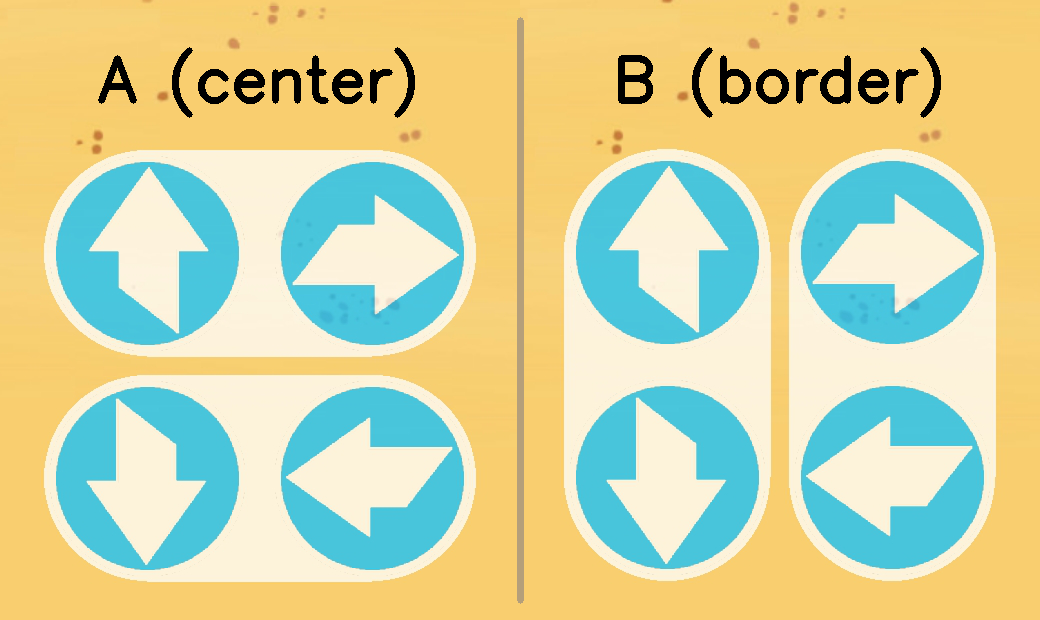
\includegraphics[width=1\linewidth]{rw-game/controls} \\ (а)
    \end{minipage}
    \hfill
    \begin{minipage}[b][][b]{0.49\linewidth}\centering
        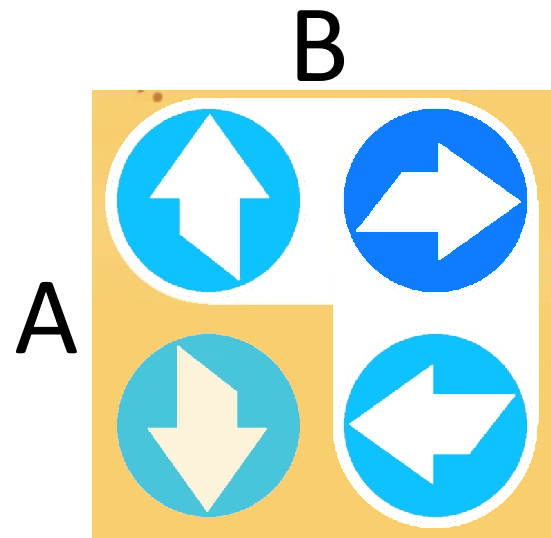
\includegraphics[width=0.73\linewidth]{rw-game/fig1e} \\ (б)
    \end{minipage}
    \caption{
        (а) Кнопки управления для игрока А, целью которого является удержание фишки внутри поля как можно дольше (центр), и для игрока Б, целью которого является скорейшее достижение границы. (б) Пример определения выбора результирующего движения фишки: игрок А выбрал первую строку (кнопку), ограничив движение направлениями вверх и вправо, игрок Б выбрал второй столбец, ограничив направления вправо и влево. В результате таких выборов игроков направление, которое выбрали оба игрока, оказывается на пересечении соответствующих столбца и строки, что дает итоговое направление движения -- вправо.
    }
    \label{fig:controls}
\end{figure}


\begin{figure}[ht]
    \centerfloat{
        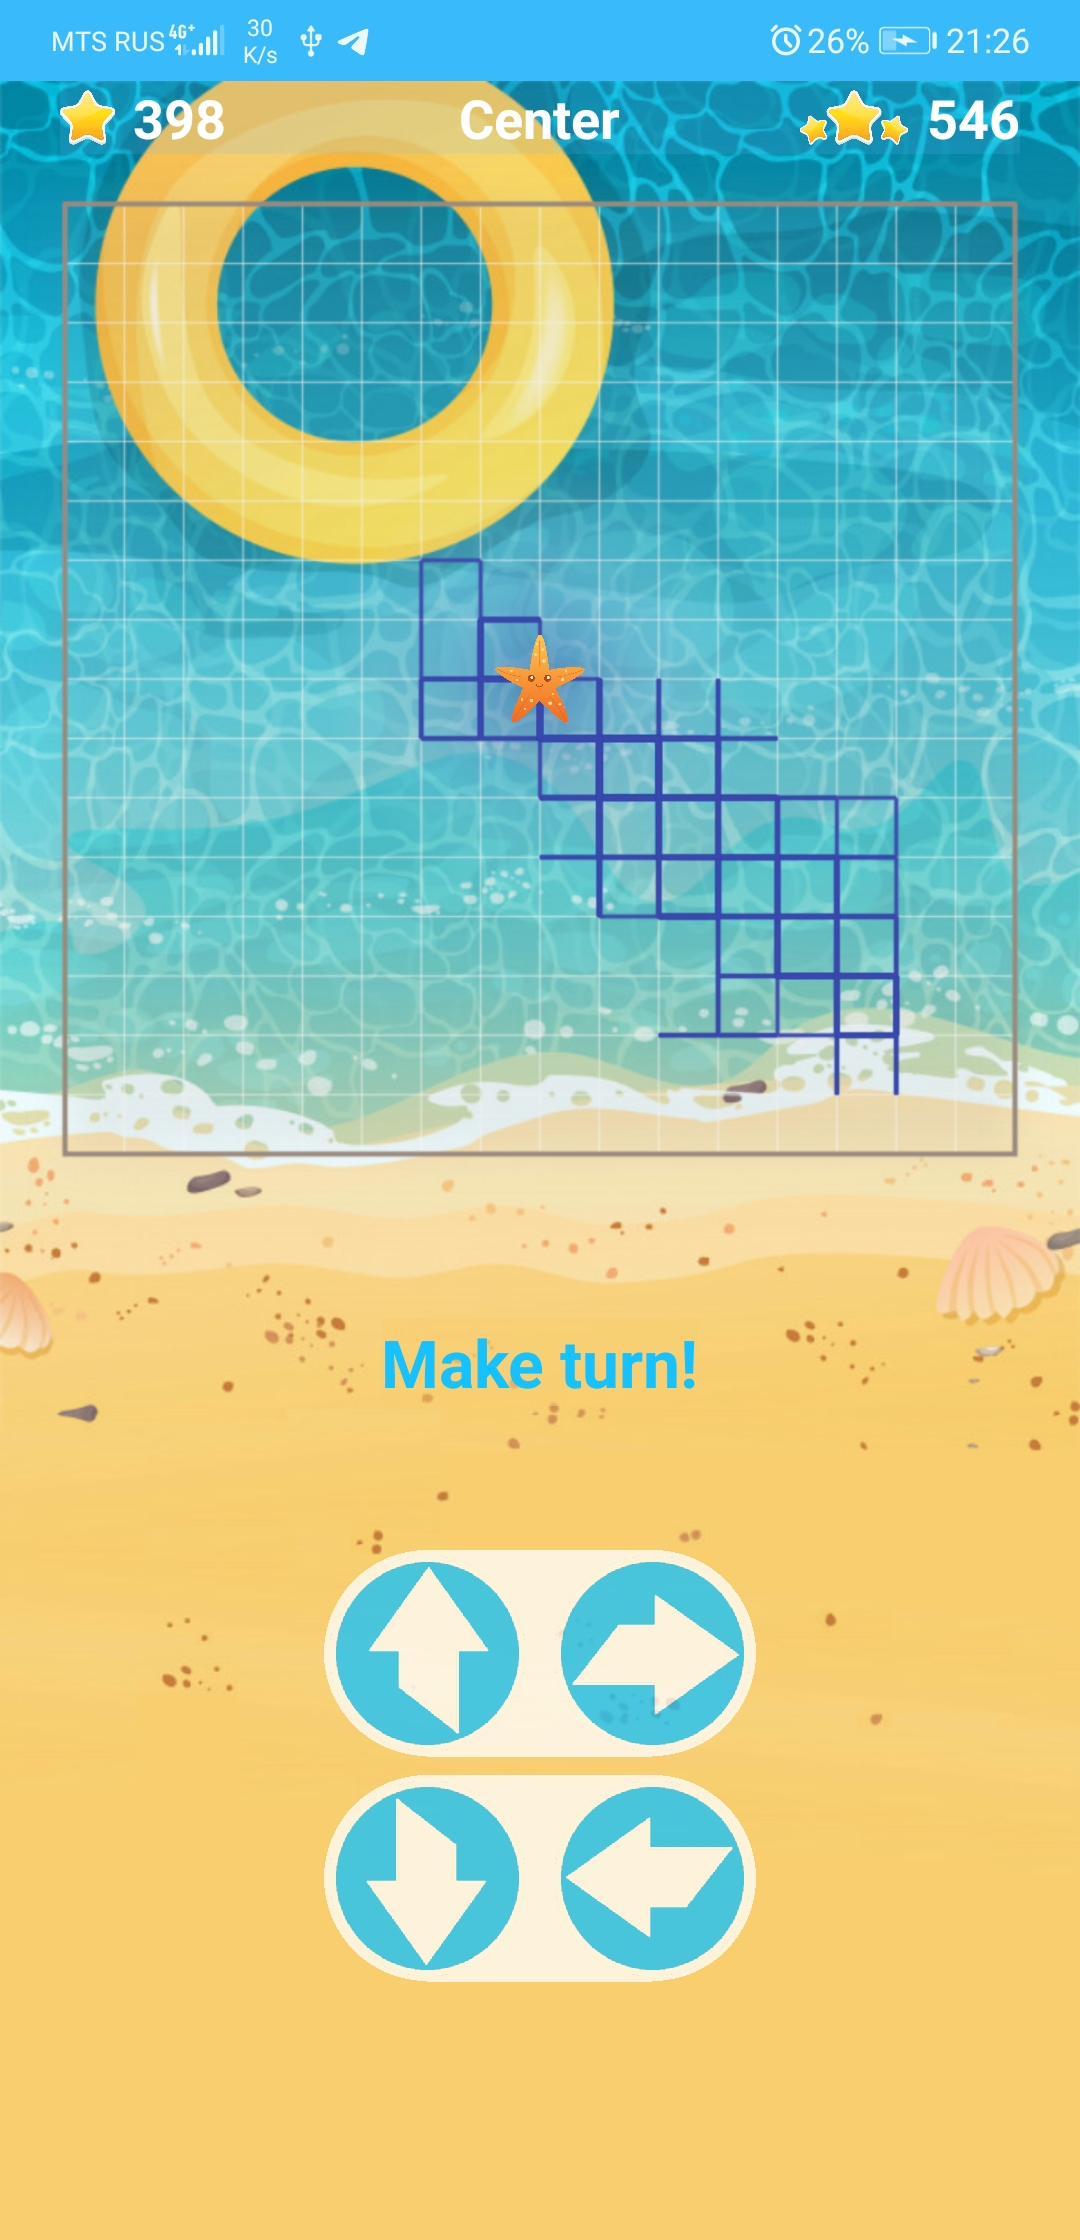
\includegraphics[scale=0.25]{rw-game/screenshot_game_field}
    }
    \caption{
        Скриншот приложения Random Walk Game. Строка заголовка состоит из текущего количества ходов, целей игроков и количества ходов в самой длинной игре. Игрок видит игровое поле, положение фишки и траекторию фишки. Внизу экрана показана управляющая матрица $2$ на $2$, которая определяет результат совместного выбора стратегий игроками A и B. Строки представляют собой возможный выбор стратегий для игрока A, а столбцы -- для игрока B. Результирующее направление движения определяется стрелкой в ячейке, расположенной в соответствующих строке и столбце.
    }\label{fig:screenshot_game_field}
\end{figure}


Рассмотренные методы в предыдущей главе для численного моделирования процесса, моделирования эволюции вероятности и расчета фундаментальной матрицы были реализованы на языке Python 3.8. Применяя данные методы были вычислены статистические свойства и распределения, рассмотренные в разделе \cref{subsec:ch3/sec2/sub2} <<Моделирование эволюции вероятности>>, для сравнения с модельной и экспериментально полученной статистикой. Расчет трех подходов (численное моделирование, моделирование вероятностной эволюции, расчет фундаментальной матрицы) и их статистические свойства были выполнены на рабочей станции (Core i5-8600 3,1 ГГц, 32 ГБ ОЗУ). Исходный код программы обсчета доступен в репозитории на GitHub \cite{RWAnalyzer}.

Результаты рассматривают игру двух оппонентов на квадратной решетке для различных случаев: BvB -- случайное блуждание на квадратной решетке, PvP -- игра между двумя игроками, PvE игра за центр против компьютера, PvE игра за границу против компьютера. Сравнение с экспериментально полученными траекториями осуществлялось на поле $17 \times 17$ в играх с реальными игроками. Выбор размера поля был определен на основе наблюдений за игроками при игре на различных размерах поля. Анализ показал, что уменьшение размера поля приводит к быстрому завершению игры, что не дает игрокам находить качественные сложные стратегии. При увеличении размера поля игры длятся слишком долго, что вызывает усталость, снижение концентрации. Это в свою очередь ведет к уменьшению заинтересованности игрока, цель которого оставаться внутри поля, в длительном матче, а также к фрустрации оппонента играющего за границу из-за многочисленных неудач. Вариант игры на поле $17 \times 17$ демонстрирует среднее время игры $10$-$15$ минут, что позволяет игрокам оставаться вовлеченными в процесс и придерживаться своих целей. Однако, длительные игры более часа также возникают в процессе проведения эксперимента. Дополнительный анализ таких игр также был проведен в рамках настоящей диссертационной работы.

Суммарно, играя в Random Walk Game, участники эксперимента провели около $250$ часов для создания исследуемого набора траекторий. В результате было получено $1562$ траектории позиции фишки на поле и соответствующих выборов игроков для трех режимов игры. Дополнительно была собрана информация о времени совершения хода каждым из игроков. В разделе \cref{sec:ch3/sec4} <<Статистические свойства игры и сравнение с экспериментом>> проводится анализ статистических свойств полученных траекторий и стратегий игроков, а также их сравнение с результатами численного анализа, моделирования и аналитических расчетов. Дополнительно приведен анализ популяционных стратегий игроков, собранных в эксперименте.

\section{Методы исследования игровых случайных блужданий}\label{sec:ch3/sec2}

Предложенная игровая динамика предполагает наличие двух игроков, осуществляющих свой выбор на каждом ходу исходя из некоторой стратегии. Одним из вариантов стратегии игроков может выступать случайный равновероятный выбор одной из кнопок на каждом ходу. Применение такой стратегии обоими игроками сводит игру к чистому случайному блужданию на ограниченной решетке -- обозначим такой случай как BvB (Bot vs Bot). Второй вариант состоит в игре человека, применяющего произвольную стратегию, против стратегии равновероятного выбора независимо от состояния -- обозначим как PvE (Player vs Environment). В этом случае различаются две стороны игры в зависимости от цели: как можно скорее достичь границу (игра за границу) и как можно дольше оставаться внутри поля (игра за центр). Последний рассмотренный вариант состоит в игре двух игроков, выбирающих произвольные стратегии (PvP -- Player vs Player).

\nomenclature{BvB}{Bot vs Bot}
\nomenclature{PvE}{Player vs Environment}
\nomenclature{PvP}{Player vs Player}

\subsection{Поглощающие Марковские цепи}\label{subsec:ch3/sec2/sub1}

Основным математическим подходом к анализу игровой динамики была выбрана теория цепей Маркова \cite{gagniuc_markov_2017}. Цепь Маркова характеризует дискретный (во времени) случайный процесс, в котором вероятность наступления каждого события зависит только от состояния, достигнутого в предыдущем событии. Представим состояние цепи в игре вектором координат положения фишки на квадратной решетке $w_k = (x_k, y_k)$ на $k$-м ходе, при этом координаты находятся в пределах:
\begin{equation}
    -\lfloor n/2 \rfloor \leq x_k \leq \lfloor n/2 \rfloor, -\lfloor n/2 \rfloor \leq y_k \leq \lfloor n/2 \rfloor. 
    \label{eq:all-states}    
\end{equation}

Всего в полученной цепи имеется $n^2-4$ достижимых узлов, $r=4(n-2)$ из которых соответствуют поглощающим (граничным) состояниям множества 
\begin{equation}
    \textbf{S}_{abs} = \{(x,y) : |x|=\lfloor n/2 \rfloor \lor |y|=\lfloor n/2 \rfloor\}
    \label{eq:border-states}
\end{equation}
и остальные $s=(n-2)^2$ -- переходным (внутренним) состояниям 
\begin{equation}
    \textbf{S}_{tr} = \{(x,y): |x|<\lfloor n/2 \rfloor \land |y|<\lfloor n/2 \rfloor\},
    \label{eq:inner-states}
\end{equation}
см. Рис.~\cref{fig:game_field}. 

Хотя существует 2 случая четности размера решетки, в работе рассмотрены только нечетные размеры, при которых начальное состояние расположено в центре поля и решетка обладает симметриями относительно центра. Минимально возможный размер такого игрового поля $3 \times 3$. 

Описание цепи в теории Марковских цепей представляется в виде матрицы переходов \cite{kemeny_finite_1976} $\mathsf{P}$ с элементами, соответствующими вероятностям $P((i, j) \rightarrow (x, y))$ изменения состояния из $(i, j)$ в $(x, y)$.

\begin{figure}[ht]
    \centerfloat{
        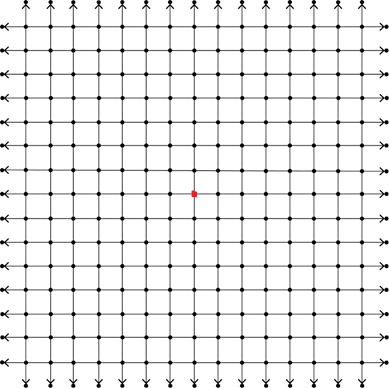
\includegraphics[width=0.5\linewidth]{rw-game/game_field}
    }
    \caption{
        %Решетка игрового поля, состоящая из внутренних узлов (серые) и граничных узлов (красные), по достижении которых происходит завершение игры.
        Решетка игрового поля, состоящая из внутренних узлов и граничных узлов, по достижении которых происходит завершение игры. Стартовый узел отмечен в центре симметричного поля нечетного размера $17 \times 17$.
    }\label{fig:game_field}
\end{figure}

Теория поглощающих Марковских цепей предоставляет возможности для расчета статистики времен поглощения \cite{kemeny_finite_1976}. В теории поглощающих Марковских цепей матрица переходов $\mathsf{P}$ представляется в виде блочной матрицы:
\begin{equation}
    \begin{aligned}
    \mathsf{P}=
      \begin{bmatrix}
        Q & R \\
        \textbf{0} & I_r
      \end{bmatrix},
    \label{eq:P}
    \end{aligned}
\end{equation}
где $Q$ это матрица размера $s \times s$, характеризующая переходы между внутренними состояниями, 
$R$ -- ненулевая матрица размера $s \times r$, соответствующая переходам из внутренних состояний в поглощающие, $I_r$ -- единичная матрица размера $r \times r$, описывающая свойство петель в поглощающих состояниях, совместно с нулевой матрицей $\textbf{0}$ размера $r \times s$, указывающей на невозможность выхода из поглощающего состояния (поглощение) \cite{kemeny_finite_1976}.

Применяя многократно матрицу переходов для внутренних состояний и проводя суммирование результирующей матрицы по всем моментам времени, теория поглощающих Марковских цепей вводит понятие фундаментальной матрицы $N$. Так как матрица $Q$ имеет норму меньшую единицы и является сжимающим отображением, то соответствующий ряд сходится и имеет место следующая замкнутая форма вычисления фундаментальной матрицы:
\begin{equation}
    N=\sum_{k=0}^{\infty} Q^k=(I_s-Q)^{-1},
    \label{eq:N}
\end{equation}
где $I_s$ это единичная матрица размера $s \times s$. Элемент фундаментальной матрицы $N$ с индексами $(i, j)$ является математическим ожиданием количества раз обнаружить цепь в состоянии $j$, при условии начала блуждания в состоянии $i$.

Используя свойство фундаментальной матрицы теория дает способ вычислить ожидаемое число шагов до поглощения при условии начала блуждания в некотором внутреннем состоянии $i$:
\begin{equation}
    \begin{aligned}
    T=N\textbf{1},
    \label{eq:T}
    \end{aligned}
\end{equation}
где $\textbf{1}$ вектор все элементы которого единицы.

В рассматриваемой игровой механике стартовая позиция игры находится в центре решетки. Тогда соответствующее математическое ожидание числа ходов до поглощения $\boldsymbol{\mathsf{t_n}}$ ($n$ -- размер поля) будет записано в элементе вектора $T$, соответствующем состоянию цепи с положением $(0, 0)$ на игровой решетке.

Игровая механика Random Walk Game предполагает игру двух оппонентов, на каждом ходу определяющих свой выбор одного из двух доступных вариантов. В общем случае, каждый из игроков обладает памятью и может ориентироваться на предысторию ходов оппонента. Формулировка игры в виде Марковского процесса позволяет одному из игроков вычислить равновесие Нэша в смешанных стратегиях \cite{nash_non-cooperative_1951}. Наличие такого равновесия и независимость стратегии от номера хода одного игрока не позволит другому игроку использовать предысторию ходов для получения большего выигрыша в среднем. Таким образом при оптимальной игре обоих игроков процесс будет являться Марковским.

Рассмотрим подробнее математическую формулировку в терминах поглощающих Марковских цепей игры Random Walk Game. Независимая от номера хода стратегия игрока $S_{ij}^p$ описывается распределением Бернулли $\sigma_{ij}^p$ для игрока $p \in \{A, B\}$ в состоянии с координатами $(i, j)$:
\begin{equation}
    \begin{aligned}
    \boldsymbol{\sigma}_{ij}^p(s)=
    \begin{cases}
        f_{ij}^p, &\mbox{if } s = 0,\\ 
        1-f_{ij}^p, &\mbox{if } s = 1,\\
    \end{cases}
    \label{eq:sigma}
    \end{aligned}
\end{equation}
где $0 \leq f_{ij}^p \leq 1$ -- вероятность выбора игроком первого варианта хода $(s=0)$.

Определение движения фишки на поле осуществляется после выбора обоими игроками своего варианта хода в соответствии с правилами, описанными в разделе \cref{subsec:ch3/sec1/sub1} <<Описание игры>> и на Рис.~\cref{fig:controls}. Движение возможно в одном из 4 направлений в соседние состояния: $(i, j + 1), (i + 1, j), (i, j - 1), (i - 1, j)$. Результирующее направление определяется совместным распределением, задающим вероятность перехода из состояния $(i, j)$ в состояние $(x, y)$:
\begin{equation}
    \begin{aligned}
    P& \left( (i, j) \rightarrow (x, y) \right) = \\
    &=\begin{cases}
        0, &\mbox{if } |i-x|+|j-y| \neq 1,\\ 
        f_{ij}^A \left(1-f_{ij}^B\right), &\mbox{if } x=i \land y=j+1, \boldsymbol{\rightarrow}\\
        \left(1-f_{ij}^A\right) f_{ij}^B, &\mbox{if } x=i+1 \land y=j, \boldsymbol{\downarrow}\\
        \left(1-f_{ij}^A\right) \left(1-f_{ij}^B\right), &\mbox{if } x=i \land y=j-1, \boldsymbol{\leftarrow}\\
        f_{ij}^A f_{ij}^B, &\mbox{if } x=i-1 \land y=j, \boldsymbol{\uparrow}\\
    \end{cases}
    \label{eq:transition}
    \end{aligned}
\end{equation}

Первый случай в формуле определяет нулевую вероятность перехода между несвязанными состояниями, и оставшиеся соответствуют четырем направлениям движения фишки.

Наборы значений $f_{ij}^p$ для двух игроков $(p \in \{A, B\})$ задают их стратегии в каждом узле квадратной решетки $(i, j)$. Фиксация этих значений до начала игры позволяет вычислить матрицу вероятностей переходов между состояниями, то есть полностью определить Марковскую цепь. Наиболее общий случай игры PvP позволяет обоим игрокам задавать свой набор вероятностей $f_{ij}^p$. В случае игры против среды PvE стратегия одного из игроков известна и представляет собой равновероятный выбор среди двух возможных вариантов независимо от позиции на поле и номера хода: $f_{ij}^{p_1} = 0.5, (p_1 \in \{A, B\})$, а для второго игрока значения определяются произвольно $f_{ij}^{p_2}, (p_2 \in \{A, B\} \setminus \{p_1\})$. Вырожденный случай игры BvB случайного блуждания определяется равновероятным выбором обоих игроков одного из вариантов хода $f_{ij}^{A} = f_{ij}^{B} = 0.5$ для всех состояний игры. В этом случае вероятность перехода из каждого внутреннего состояния в соседнее равно $\frac{1}{4}$.

Оба игрока рассматривают в качестве цели количество ходов в игре. Цель одного минимизировать количество ходов, а цель второго -- максимизировать. В случае Марковской цепи при определенных смешанных стратегиях игроков целевой функцией является математическое ожидание времени достижения границы. Обозначим соответствующие средние времена поглощения в игре для 4 случаев как $\boldsymbol{\mathsf{t_n^{BvB}}}$, $\boldsymbol{\mathsf{t_n^{PvEA}}}$, $\boldsymbol{\mathsf{t_n^{PvEB}}}$ и $\boldsymbol{\mathsf{t_n^{PvP}}}$.

\subsection{Моделирование эволюции вероятности}\label{subsec:ch3/sec2/sub2}

Аналитический подход теории поглощающих Марковских цепей позволяет вычислить значение среднего времени поглощения случайного блуждания с применением матричных преобразований. Однако теории для расчета точного распределения времени поглощения в случае Марковских цепей в замкнутой форме автору не известно. Прямой подход к расчету оценки распределения времени поглощения возможен благодаря математическому моделированию процесса эволюции вероятности. Дополнительным преимуществом данного подхода является возможность оценки наряду с распределением времени достижения также пространственного распределения вероятностей. 

Рассмотрим подробнее модель эволюции вероятности. Пусть $W_{ij}^{k}$ -- вероятность найти фишку в состоянии $(i, j)$ в момент времени $k$. Начальное состояние игры в центре поля $(0, 0)$ соответствует единичной вероятности найти частицу в начальный момент времени $t=0$ в состоянии $(0, 0)$, то есть $W_{0,0}^{0}=1$ и $W_{ij}^{0}=0$ для остальных состояний $((i, j) \neq (0, 0))$. Упорядочим все состояния последовательно по формуле $in + j$, где $n$ -- размер поля. Тогда вектор $\boldsymbol{w^{0}}$ описывает распределение вероятности в начальный момент времени, а для всех моментов времени $k > 0$ распределения последовательно определяются по формуле эволюции вероятности:
\begin{equation}
    \begin{aligned}
    \boldsymbol{w^{k+1}}=\mathsf{\widetilde{P}}\boldsymbol{w^{k}}, k \geq 0,
    \label{eq:evolution}
    \end{aligned}
\end{equation}
где $\mathsf{\widetilde{P}}$ -- модифицированная матрица вероятностей переходов между состояниями цепи. 

Эволюция вектора вероятности на каждом шаге также дает возможность оценить точную вероятность $W_{ij}^{k}, (i, j) \in \boldsymbol{B}$ окончания блуждания на $k$-ом ходу в граничном состоянии $(i, j)$. Для этого используется модифицированная матрица переходов такая, что при достижении границы фишкой происходит ее исключение из системы. Тогда вероятность поглощения частицы на $k$-ом шаге может быть вычислена по следующей формуле:

\begin{equation}
    \begin{aligned}
    p_\mathsf{abs}^{k}=\sum_{(i, j) \in \boldsymbol{\mathsf{B}}} W_{ij}^{k},
    \label{eq:timedistr}
    \end{aligned}
\end{equation}
где $\textbf{B}$ -- множество граничных состояний.

Моделирование эволюции вероятности также позволяет вычислить пространственное распределение вдоль граничных состояний за счет аппроксимации ряда вероятностей поглощения в узле $(i, j) \in \boldsymbol{\mathsf{B}}$ по всем моментам времени:
\begin{equation}
    \begin{aligned}
    p_{ij}^\mathsf{abs}=\sum_{k=0}^{\infty} W_{ij}^{k}
    \label{eq:spacedistr}
    \end{aligned}
\end{equation}

В связи с экспоненциальным убыванием вероятности $W_{ij}^{k}$ с ростом номера $k$ суммирование выполняется до достижения заданной точности модуля разности между соседними членами.

Дополнительным свойством, представляющем интерес при анализе игровой динамики, является соотношение вероятностей закончить игру на четном числе ходов или на нечетном. Отличие этого соотношения от единицы обусловлено тем, что квадратная решетка представляет собой двудольный граф, в связи с чем на каждом ходу фишка может находиться только в одной из долей в зависимости от четности хода. Обозначим долю графа четной, если фишка находится в ней на четном ходу, и нечетной -- если на нечетном ходу. Состояния $(i, j)$ двух долей расположены на решетке в шахматном порядке и аналогично могут быть отнесены к "четным" и "нечетным" состояниям в соответствии с четностью суммы координат $(i + j) \mod 2$. Распространение вероятности по цепи происходит за счет полного перехода между долями. Однако вероятность поглощения в четных и нечетных состояниях отличается ввиду разного количества и расположения поглощающих состояний в долях.

Применение подхода к моделированию эволюции вероятности позволяет численно получить большой спектр информации о свойствах игры.

Анализ статистических свойств игровой динамики возможен благодаря подходам, использующим теорию Марковских цепей и моделирование эволюции вероятности. Однако исследование структурных особенностей индивидуальных траекторий требует применения методов численного моделирования. Одним из способов решения задачи является метод Монте-Карло для симуляции случайного процесса с использованием генератора случайных чисел. Сталкивая различные смешанные стратегии, исследуемые в ходе работы, возможно построить последовательность перемещений фишки по решетке, движущейся в соответствии с правилами игры. Алгоритм симуляции состоит из нескольких шагов:
\begin{itemize}
\item Начальное положение фишки определяется в центре поля $(0, 0)$. 
\item На каждом ходе генерируются выборы игроков из распределения с соответствующей стратегией игрока с использованием псевдослучайного генератора Mersenne Twister \cite{matsumoto_mersenne_1998} из модуля random в Python 3.8.
\item В соответствие с правилами перехода фишка перемещается в одно из соседних состояний.
\item По достижении фишкой одного из граничных состояний симуляция останавливается.
\end{itemize}

В результате работы алгоритма генерируется последовательность ходов игроков и движений фишки на поле. Для визуализации индивидуальных траекторий реализованы три способа: 
\begin{itemize}
\item визуализация всех ходов траектории с наложением на одной плоскости;
\item разбиение ходов на последовательные группы по 40 ходов и визуализация групп блоками от первой до очередной группы;
\item анимация движения фишки и след траектории с затуханием.
\end{itemize}

Дополнительно, при сравнении с результатами моделирования эволюции вероятности были вычислены частоты встречаемости времен полученных игр (эмпирическая функция вероятности). 

\subsection{Полевой эксперимент с применением мобильных приложений и сети интернет}\label{subsec:ch3/sec2/sub3}

Математический подход к анализу стратегий дает возможность выявить наиболее оптимальные способы действия игроков. Однако в реальных условиях на поведение человека, принимающего решение о конкретном ходе, влияет большой спектр факторов: настроение, предыдущие действия игроков, внешние обстоятельства, индивидуальный когнитивный статус и другие факторы. Естественный подход к продолжению анализа игровой динамики состоит в проведении полевого эксперимента с участием людей в качестве игроков. 

Для участия в эксперименте были приглашены волонтеры в возрасте от 16 до 52 лет. Игроки до 25 лет были отобраны из числа студентов ННГУ им. Н.~И.~Лобачевского и Высшей школы экономики. Игроки старше 25 лет были набраны из разных университетов и исследовательских институтов России, Германии, Норвегии и Южной Кореи.

Основной критерий для отбора участников состоял в основном роде деятельности заключающемся в умственном труде. Большая часть участников представляет собой успешных студентов, призеров олимпиад, профессоров, кандидатов наук, успешных ИТ-специалистов.

Проведение эксперимента состояло из четырех отдельных мероприятий:
\begin{itemize}
\item Организованные игры без конкурса между участниками. Студенты находились в одной комнате и играли не общаясь друг с другом в течение одного часа. Интерес участников заключался в достижении самой длинной игры среди участников. Пары игроков выбирались на основе схожести их навыков в олимпиадном программировании.
\item Конкурс на получение наибольшего количества очков при игре против среды PvE. Участники играли онлайн в течение месяца соревнуясь с другими участниками в общем рейтинге. Рейтинг представлял собой отношение двух экспоненциально скользящих средних длительностей по играм за центр и за границу. Общий рейтинг все время был доступен участникам.
\item Личный чемпионат между студентами в играх PvP. Студенты находились в одной аудитории и играли не общаясь друг с другом в течение двух часов. Участники распределялись по взвешенной сумме длин сыгранных игр. Чем длиннее игра -- тем выше вес, связанный с этой игрой для участника, играющего за центр (A) и противоположный для участника, играющего за границу (B). Интерес участников заключался в получении наивысшего места в таблице.
\item Свободные игры без конкурса между участниками и между участником и средой. Участники находились дома и играли не общаясь около 30 минут в день. Интерес участников состоял в получении наибольшего (наименьшего) счета в конкретной игре. В любой момент игроки могли приостановить игру и продолжить ее в удобное для них время.
\end{itemize}

Цели игроков распределялись между ними равновероятно на основе генератора случайных чисел. В результате реализации эксперимента было собрано 500 игр типа PvP, 500 игр типа PvE за центр и 500 игр типа PvE за границу.

Для организации экспериментальной части было разработано мобильное приложение, доступное в Google Play Store \cite{googleplay} и в App Store \cite{applestore}. Приложение предоставляет два режима игры: игра против другого игрока (PvP) или игра против среды (PvE). В обоих режимах приложение отправляет выбор игроков через Интернет на веб-сервер и рассчитывает направление и следующую позицию фишки на поле. Результаты игр (траектории и соответствующие выборы стратегий игроков на каждом ходу) были собраны в базе данных на сервере для дальнейшего анализа. Основной экран мобильного приложения с игровым полем представлен на Рис.~\cref{fig:screenshot_game_field}.

Выбор одной из двух стратегий среды в режиме PvE определяется последовательностью псевдослучайных чисел, вычисленных генератором случайных чисел Mersenne Twister (реализованным в PHP 7.4 как функция $\mathsf{mt\_rand}$) \cite{matsumoto_mersenne_1998}. Игры, полученные в эксперименте, проводились на поле размера $17 \times 17$.

Архитектура системы состоит из трех основных компонент: мобильное приложение, веб-сервер и база данных. Взаимодействие между мобильным приложением и веб-сервером осуществляется посредством REST API по защищенному протоколу HTTPS через сеть Интернет. Процесс взаимодействия клиента и сервера состоит из нескольких этапов:
\begin{itemize}
\item Пользователь осуществляет регистрацию в системе, информация о регистрации отправляется на веб-сервер и сохраняется в базу данных (БД).
\item Пользователь аутентифицируется в системе на основе связки логин и пароль, либо на основе OAuth аутентификации.
\item Успешная аутентификация авторизует пользователя в системе и предоставляет список текущих игр пользователя, историю игр пользователя, рейтинг участников, и возможность начать новую игру.
\item Игрок инициирует игру с другим игроком по логину, случайным образом или выбором незавершенной игры из списка.
\item После инициализации двумя игроками одной и той же игры, выбранная каждым игроком стратегия на ходе передается на веб-сервер и сохраняется в БД.
\item Клиент опрашивает веб-сервер до тех пор, пока оба игрока не совершат выбор в текущем ходе.
\item После совершения выбора обоими игроками веб-сервер определяет направление движения фишки, факт достижения границы и по запросу передает на мобильное устройство эту информацию.
\item На клиенте обновляется положение фишки, количество ходов. Игра переходит на следующий ход или завершается.
\end{itemize}

\nomenclature{REST API}{Representational state transfer Application Programming Interface}
\nomenclature{БД}{База данных}

В качестве HTTP-сервера используется веб-сервер nginx \cite{reese_nginx_2008}. Программная часть, реализующая функционал серверной части, разработана на языке PHP 7.4 \cite{Nixon_web_2016} без использования дополнительных фреймворков с использованием модели Model-View-Controller (MVC) \cite{pitt_pro_2021}. Хранение информации реализовано на основе реляционной базы данных MySQL с применением хранимых процедур для защиты от XSS атак к базе данных \cite{stuttard_web_2011}. Защита паролей осуществляется с применением хеширования с солью на основе алгоритма bcrypt (реализовано в PHP 7.4 как функция $\mathsf{password\_hash}$).

\nomenclature{XSS}{Cross Site Scripting}
\nomenclature{MVC}{Model-View-Controller}

Мобильное приложение разработано с применением технологии Xamarin на языке C$\mathsf{\#}$ \cite{sole_xamarin_2022}. Преимуществом данной технологии в сравнении с другими, такими как Kotlin в среде разработки Android Studio, Objective-C, Swift в среде разработки XCode, является кроссплатформенность при сохранении общей кодовой базы бизнес-логики и возможности индивидуализации интерфейса пользователя по конкретную платформу. Xamarin предлагает три платформы для сборки приложения: Universal Windows App, Android, iOS. Наличие широкого выбора компонент, оптимизированных для разных платформ, позволило в короткие сроки разработать мобильное приложение для трех платформ. Основным паттерном проектирования приложения был выбран подход Model-View-ViewModel (MVVM). Разделение приложения на логически связанные компоненты и построение качественной архитектуры позволило сделать приложение гибким к внесению дополнительных изменений.

\nomenclature{MVVM}{Model-View-ViewModel}

\section{Поиск оптимальных стратегий}\label{sec:ch3/sec3}

Основной целью для игроков является увеличение или уменьшение количества ходов, за которое будет достигнута граница поля. Однако, особенность рассматриваемой игры состоит в наличии случайной компоненты, не зависящей напрямую от игроков и лежащей в основе механики их взаимодействия. Для исключения влияния случайной компоненты на результирующий функционал был предложен подход к оценке среднего количества ходов, за которое фишка достигнет границу поля (среднее время игры). Применение такого подхода позволяет находить оптимальные стратегии, дающие максимум или минимум среднего времени игры в зависимости от цели игрока.

В данном разделе рассматривается 4 случая игры: вырожденный случай, 2 случая игры против бота, и случай игры двух игроков, оптимизирующих своих стратегии. Для каждого случая приводятся оценки средних времен поглощения, при оптимальной игре. С использованием теории Марковских цепей и теории рекурсивных игр находятся оптимальные стратегии игры.

\subsection{Вырожденный случай BvB неуправляемого случайного блуждания}\label{subsec:ch3/sec3/sub1}

Рассмотрим особый вырожденный случай игры, сводящийся к случайным блужданиям на плоскости. В данном случае (BvB) игроки совершают равновероятный выбор на каждом ходу одного из двух выборов, то есть среднее время игры зависит только от размера поля. Применяя метод расчета фундаментальной матрицы для поглощающей Марковской цепи для разных размеров поля были получены значения среднего времени игры для случая BvB. Используя аппроксимацию квадратичной зависимостью на основе метода наименьших квадратов (МНК) зависимости среднего времени для размеров полей в диапазоне от $3$ до $1001$
были получены численные коэффициенты параболы: $\boldsymbol{\mathsf{t_n^{BvB}}} = 0.294685413 n^2 - 0.232$ (Рис.~\cref{fig:quadratic:time}). Средняя абсолютная ошибка аппроксимации составила $10^{-3}$. 

Хотя простого способа представления в замкнутой форме данной зависимости  не было найдено, в работе \cite{kmet_gamblers_2002} была предложена форма из нескольких сумм, позволяющая оценить
среднее время игры для случая BvB, как простого случая случайного блуждания на ограниченном квадрате. Однако, для нашего случая $N=16$, то есть степени 2, была получена формула в виде одной суммы:
\begin{equation}
	\begin{aligned}
		& \overline{k}_N^{BvB} = \frac{2}{N} \sum_{k=0}^{N/2-1} (-1)^k \alpha_{k,N} 
		\frac{\cos((2k+1)\pi/(2N))}{\sin^3{(2k+1)\pi/2N}}, \\
		% &0 \leq i, j \leq N, \\
		\alpha_{k,N} =& 1-\frac{1}{\cosh(N/2)\cosh^{-1}\left(1+2\sin^2\frac{(2k+1)\pi}{2N}\right)}.
		\label{eq:absorption_bvb_center}
	\end{aligned}
\end{equation}
Вычисление выражения также дает среднее время случайного блуждания $75.22$ при $N=16$ при старте в центральном узле.

\subsection{Задача глобальной оптимизации для случая PvE}\label{subsec:ch3/sec3/sub2}

Рассмотрение случаев PvE приводит к необходимости поиска оптимальных стратегий. В связи с этим возникает постановка задачи математического программирования по глобальной оптимизации среднего времени игры в пространстве стратегий. Как было рассмотрено в разделе \cref{subsec:ch3/sec2/sub1} <<Поглощающие Марковские цепи>> в соответствии с формулой \eqref{eq:transition} функция среднего времени игры зависит от двух векторов с вещественными элементами из диапазона $[0, 1]$, характеризующих стратегии каждого из игроков. В случае PvE стратегия одного из игроков фиксирована и может быть исключена из аргументов задачи оптимизации. Тогда возникают две независимые задачи оптимизации для случаев игры за центр и за границу:
\begin{equation}
    \begin{aligned}
        \boldsymbol{\mathsf{t_n^{PvEA}}} = \max_{f^A \in \boldsymbol{\mathsf{F}}} \boldsymbol{\mathsf{t_n}}, \hspace{1em} f_{ij}^B=1/2,
    \label{eq:centeropt}
    \end{aligned}
\end{equation}
\begin{equation}
    \begin{aligned}
        \boldsymbol{\mathsf{t_n^{PvEB}}} = \min_{f^B \in \boldsymbol{\mathsf{F}}} \boldsymbol{\mathsf{t_n}}, \hspace{1em}  f_{ij}^A=1/2,
    \label{eq:borderopt}
    \end{aligned}
\end{equation}
где $\boldsymbol{\mathsf{F}}$ -- пространство векторов с элементами в диапазоне $[0, 1]$, которые соответствуют выбранным относительным частотам $f_{ij}^p$ в смешанных стратегии игрока $p \in [A, B]$. Расчет $\boldsymbol{\mathsf{t_n}}$ осуществляется с применением рассмотренного подхода поглощающих Марковских цепей в разделе \cref{subsec:ch3/sec2/sub1} <<Поглощающие Марковские цепи>> с использованием формул \eqref{eq:P}, \eqref{eq:N}, \eqref{eq:T}, \eqref{eq:transition}.

Количество переменных в задаче оптимизации растет квадратично с ростом размера поля, что существенно усложняет анализ для выбранных размеров $17 \times 17$. Однако для случаев с небольшим числом оптимизируемых переменных задача может быть решена напрямую поиском глобального оптимума. Применяя алгоритм \texttt{Minimize} математического пакета Wolfram Mathematica для решетки размеров $5$ и $7$ удалось получить значения оптимального времени игры для случаев игры против случайного равновероятного выбора компьютером (PvE), а также набор найденных стратегий. Случай $3 \times 3$ не представляет прямого интереса, так как среднее время поглощения равно $1$ независимо от выбора стратегий игроков, так как поглощение фишки происходит на первом ходу. Случай $5 \times 5$ уже не является вырожденным и выборы игроков влияют на результат среднего времени игры. Всего при решении данного случая возникает задача оптимизации с $9$ параметрами, которая может быть решена с применением \texttt{Minimize}.

Количество параметров для решения задачи большего размера при использовании данного подхода слишком велико, что не позволяет без упрощения найти оптимальную стратегию. Для уменьшения размерности воспользуемся симметриями в игре стратегий игроков относительно главной и побочной диагоналей. Две симметрии позволяют свернуть игру уже на одном из $4$ треугольников между главной и побочной диагоналями. Для определенности выберем верхний треугольник. Тогда верхняя граница, как и ранее, соответствует граничным поглощающим состояниям, а две новые стороны треугольника соответствуют отражающим границам, то есть из состояний на диагонали возможно перейти только в $2$ соседних состояния внутри треугольника. Учет данных симметрий позволяет приблизительно в $4$ раза уменьшить количество состояний и соответственно количество различных элементов в векторе стратегий, что позволило решить задачу для случая $7 \times 7$. 

\subsection{Гипотеза об оптимальных стратегиях для случая PvE}\label{subsec:ch3/sec3/sub3}

Анализируя стратегии и значения среднего времени игры, найденные с применением глобальной оптимизации, для малых размерностей, а также учитывая свойства игры, для достижения оптимальных значений были предложены $2$ стратегии, опубликованные в тезисах конференции \cite{confbib1}. Случай PvE состоит из двух вариантов игры: с целью удержать фишку как можно дольше внутри поля (максимизировать среднее время игры) и с целью как можно скорее достичь границы (минимизировать среднее время игры). Значения оптимального среднего времени игры для обоих случаев представляют квадраты нечетных чисел для малых размеров поля. В случае PvE при игре за центр формула представляется в виде: $\boldsymbol{\mathsf{t_n^{PvE A}}} = (n-2)^2$ и в случае игры за границу в виде: $\boldsymbol{\mathsf{t_n^{PvE B}}} = \frac{(n-1)^2}{4}$. 

В предположении сохранения такой же закономерности для больших размеров поля, рассмотрим стратегии, достигающие средних времен игры $\boldsymbol{\mathsf{t_n^{PvE B}}}$ и $\boldsymbol{\mathsf{t_n^{PvE A}}}$. Принцип построения стратегии в обоих случаях состоит в выборе некоторой одномерной структуры внутри поля, на которой игрок может поддерживать блуждание без выхода за границу этой структуры. Такая структура будет представлять собой одномерную марковскую цепь, по которой игрок может осуществлять некоторое блуждание. При этом большее количество узлов цепи будет соответствовать большим средним временам. Таким образом в случае игры за центр необходимо выбрать наиболее длинную такую структуру, а в случае игры за границу наиболее короткую.

Самая длинная одномерная цепь, внутри которой игрок за центр может сохранять свою фишку независимо от выборов второго игрока, представляет собой <<лестницу>> состояний на главной диагонали. С характеристикой наиболее длинной цепи также существует побочная диагональ, однако правила игры не позволяют поддерживать случайное блуждание на ней независимо от ходов второго игрока. Для поддержания фишки на <<лестнице>> главной диагонали игрок чередует свой выбор кнопок на каждом ходу. Выбор такой структуры позволяет получить одномерную марковскую цепь длины $2n-3$, случайное блуждание вдоль которой осуществляется равновероятно в обоих направлениях, так как $f_{ij}^B=\frac{1}{2}$. Такая Марковская цепь соответствует случаю игры о разорении игрока с одной валютой. Применяя формулу для среднего времени случайного блуждания на отрезке \eqref{eq:eq6}, рассмотренную в разделе \cref{subsec:ch1/sec1/sub1} <<Задача о разорении игрока>>, получим среднее время $\boldsymbol{t_n^{PvE A}} = ((2n-3-1)/2)^2 = (n-2)^2$, соответствующее обнаруженной закономерности. График зависимости представлен на Рис.~\cref{fig:quadratic:time}.

Аналогично, применяя принцип поиска структуры одномерной цепи, выберем самую короткую цепь для случая игры за границу. Такой цепью будет являться горизонтальный или вертикальный отрезок, проходящий через центральную стартовую позицию. Независимо от выборов первого игрока, второй игрок сможет выбирая одну и ту же кнопку оставаться на данном отрезке. Полученная цепь состоит из $n$ состояний, что дает среднее время поглощения $\boldsymbol{\mathsf{t_n^{PvE B}}} = \frac{(n-1)^2}{4}$, график зависимости представлен на Рис.~\cref{fig:quadratic:time}. Игрок необязательно должен выбрать только один из отрезков, а может использовать их комбинацию, переходя в центральном узле между ними, ввиду симметрий рассмотренных в предыдущем разделе. 

Рассмотренные стратегии не являются единственными достигающими найденные значения среднего времени игры. Одна из стратегий для случая игры за центр, использующая не только одномерный набор состояний, а все игровое поле целиком, может быть сформулирована следующим образом: в состояниях соседних с граничными выбор стратегии состоит в движении от границы или вдоль нее, а во всех остальных состояниях выбор осуществляется произвольным образом. Применяя символьные вычисления Wolfram Mathematica в методе расчета среднего времени игры с использованием фундаментальной матрицы было продемонстрировано для размеров поля $5, 7, 9, 11$, что все переменные $f_{ij}^A$, соответствующие состояниям не инцидентным границе, после упрощения выражения имеют нулевые коэффициенты. Времена, получаемые при данной стратегии, также совпадают с найденной закономерностью $\boldsymbol{\mathsf{t_n^{PvE A}}}$.

Все 3 найденных зависимости среднего времени игры для трех случаев представляют собой квадратичную функцию с различными коэффициентами (Рис.~\cref{fig:quadratic:time}). Старший коэффициент при $n^2$ для случая PvE за центр -- $1$, для случая PvE за границу -- $0.25$, для случайного блуждания BvB -- $0.29$. Таким образом, оптимальная стратегия в случае PvE игры за центр показывает время в $3.4$ раза большее, чем случайный равновероятный выбор игрока в случае BvB. В случае же игры PvE за границу время оказывается меньше, чем при случайном равновероятном выборе в случае BvB, приблизительно на $15\%$.

\begin{figure}[t]
    \centering
    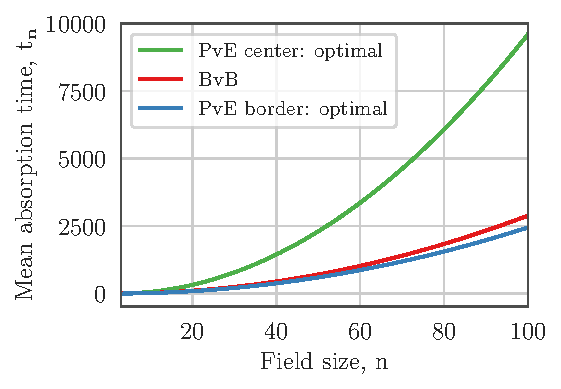
\includegraphics[width=\columnwidth,keepaspectratio,clip]{rw-game/fig2.pdf}
    \caption{
        Квадратичные зависимости среднего времени поглощения от размеров поля для случаев: центр PvE для игрока A (цель игрока оставаться внутри как можно дольше) -- зеленая линия, граница PvE для игрока B (цель игрока достичь границу как можно скорее) -- синяя линия, BvB (времена поглощения чистого случайного блуждания) -- красная линия.
    }  
    \label{fig:quadratic:time}
\end{figure}

Применение теории рекурсивных игр, подробно рассмотренной в следующем разделе \cref{subsec:ch3/sec3/sub4} <<Решение задачи поиска оптимальных стратегий>>, демонстрирует оптимальность приведенных средних времен для случаев игры против бота (PvE), что позволяет утверждать также и оптимальность предложенных стратегий.

\subsection{Решение задачи поиска оптимальных стратегий}\label{subsec:ch3/sec3/sub4}

Предложенная игра Random Walk Game может быть рассмотрена как последовательно составная игра двух оппонентов с нулевой суммой. Конкретизация свойств игры приводит к возможности ее представления в виде рекурсивной игры. На каждом этапе такой игры проводится некоторая игра в нормальной форме из набора доступных игр, в которой стратегии игроков совместно определяют платежи, вероятности каждой из доступных игр на следующем этапе, а также вероятность завершения игры \cite{luce_games_1957a}. В аналогичной форме представляются стохастические игры. Основными особенностями рекурсивных игр по сравнению со стохастическими является возможность наличия нулевых вероятностей завершения игры и произведение платежа только по окончании игры. Анализ рекурсивных игр для общего случая выполнен в работе Эверетта \cite{everett_recursive_1958}.

Представляя игру Random Walk Game в виде рекурсивной игры определим набор доступных простых игр на каждом ходу $\Gamma_{i,j}$, соответствующих внутренним состояниям $(i, j) \in \textbf{S}_{tr}$ на игровом поле. Всего таких простых игр $n^2-4$. Дополнительно определим для индексов, соответствующих поглощающим состояниям марковской цепи, $\Gamma_{i,j}=K, (i,j) \in \textbf{S}_{abs}$, где $K$ обозначает завершение игры с нулевым заключительным платежом. Последовательные вероятности переходов между простыми играми определяются в соответствии с правилами игры Random Walk Game. Тогда матрица для простой игры с индексом $(i, j) \in \textbf{S}_{tr}$ определяется следующим образом:
\begin{equation}
    \begin{aligned}
        \Gamma_{i,j}: \begin{blockarray}{ccc}
     & \mathbin\downarrow\hspace{-0.3em}\uparrow & \text{\makebox[2pt][l]{\raisebox{-5pt}{$\leftarrow$}}}\rightarrow \\
    \begin{block}{l[cc]}
        \text{\makebox[3pt][l]{\raisebox{0pt}{$\uparrow$}}}\text{\makebox[0pt][l]{\raisebox{-7pt}{$\rightarrow$}}} & \Gamma_{i-1,j} & \Gamma_{i,j+1} \\
        \text{\makebox[6pt][l]{\raisebox{6pt}{$\leftarrow$}}}\downarrow & \Gamma_{i+1,j} & \Gamma_{i,j-1} \\
    \end{block}
    \end{blockarray},
    \label{eq:recursive-game-transitions}
    \end{aligned}
\end{equation}
где элементы матрицы определяют переходы из игры, соответствующей состоянию $(i, j)$ в игры, соответствующие состояниям $(i-1, j)$, $(i, j+1)$, $(i+1, j)$, $(i, j-1)$ в исходной марковской цепи; строки матрицы задают стратегии первого игрока, играющего за центр, столбцы матрицы задают стратегии второго игрока, играющего за границу. 

Цена игры $\Gamma_{i,j}^{k}$ на $k$-ом этапе определяется как цена игры на следующем этапе плюс единица, отражающая очередной ход в игре. Тогда для цены игры можно записать:
\begin{equation}
    \begin{aligned}
        |\Gamma_{i,j}^{k}| = 1 + \left | \begin{bmatrix}
			|\Gamma_{i-1,j}^{k+1}| & |\Gamma_{i,j+1}^{k+1}| \\
			|\Gamma_{i+1,j}^{k+1}| & |\Gamma_{i,j-1}^{k+1}|
		\end{bmatrix} \right |,
    \label{eq:game-payments}
    \end{aligned}
\end{equation}
где $|\Gamma_{i,j}^k|$ обозначает цену игры $\Gamma_{i,j}$ на $k$-ом этапе.

Обозначим $\nu_{i,j}=|\Gamma_{i,j}|$ цену простой игры $\Gamma_{i,j}$. Тогда каждая простая игра представляет собой матричную игру $2\times2$ с нулевой суммой. Решением такой игры выступает набор смешанных стратегий, если седловая точка отсутствует, иначе -- набор чистых стратегий \cite{ouen_teoriya_1971}. В случае наличия седловой точки в матрице платежей, цена игры равна значению в седловой точке, а стратегии игроков выбираются так, чтобы при их выборе итог игры являлся седловой точкой. В случае отсутствия седловой точки решением игры выступает набор смешанных стратегий и цена игры может быть найдена по формуле:
\begin{equation}
    \begin{aligned}
        \left | \begin{bmatrix}
			\nu_{i-1,j} & \nu_{i,j+1} \\
			\nu_{i+1,j} & \nu_{i,j-1}
		\end{bmatrix} \right | = \frac{\nu_{i-1,j}\nu_{i,j-1} - \nu_{i+1,j}\nu_{i,j+1}}{\nu_{i-1,j} + \nu_{i,j-1} - \nu_{i+1,j} - \nu_{i,j+1}},
    \label{eq:game-2x2-value}
    \end{aligned}
\end{equation}
при этом вероятности стратегий игроков определяются выражениями:
\begin{equation}
    \begin{aligned}
        p_{i,j}^{(A)} = \frac{\nu_{i,j-1} - \nu_{i+1,j}}{\nu_{i-1,j} + \nu_{i,j-1} - \nu_{i+1,j} - \nu_{i,j+1}}, \\
        p_{i,j}^{(B)} = \frac{\nu_{i,j-1} - \nu_{i,j+1}}{\nu_{i-1,j} + \nu_{i,j-1} - \nu_{i+1,j} - \nu_{i,j+1}}.
    \label{eq:game-2x2-prob}
    \end{aligned}
\end{equation}

Рассматриваемая рекурсивная игра обладает свойством унивалентности \cite{everett_recursive_1958}, то есть имеет неотрицательные (неположительные) платежи в каждой простой игре. Дополнительно игра Random Walk Game не имеет <<ловушек>>, то есть узлов, в которых один из игроков может детерминировано оставлять фишку в течение произвольного числа ходов. В соответствии с работой Эверетта \cite{everett_recursive_1958} и книгой Льюс и Райфа \cite{luce_games_1957a} решением унивалентной рекурсивной игры без <<ловушек>> является одна из неподвижных точек преобразования цен $T$, задающегося как новый вычисленный набор цен игр на основе набора предыдущих цен. Математически преобразование цен $T$ задается следующим образом:
\begin{equation}
    \begin{aligned}
        (\nu_{i,j}) \xrightarrow{T} (\nu_{i,j}^\prime), \\
        \nu_{i,j}^\prime = \big |\Gamma_{i,j} \big(\left (\nu_{i,j} \right ) \big)\big |.
    \end{aligned}
\end{equation}

Для нахождения неподвижной точки преобразования применим численный итеративный метод, многократно применяющий отображение $T$ \cite{everett_recursive_1958}. В качестве начального набора цен выберем произвольный ненулевой вектор $\boldsymbol{\nu}_{init}$ с неотрицательными элементами. 
Итеративно применим отображение $T$ до достижения желаемой точности $\max_{i,j}\left |\nu_{i,j}^{(k)}-\nu_{i,j}^{(k+1)}\right |<\epsilon=10^{-5}$. Заданная точность была достигнута за 1000 итераций. Результирующие значения $\nu_{i,j}$ приведены на рисунке \cref{fig:optimal-value-pvp}.

\begin{figure}[t]
    \centering
    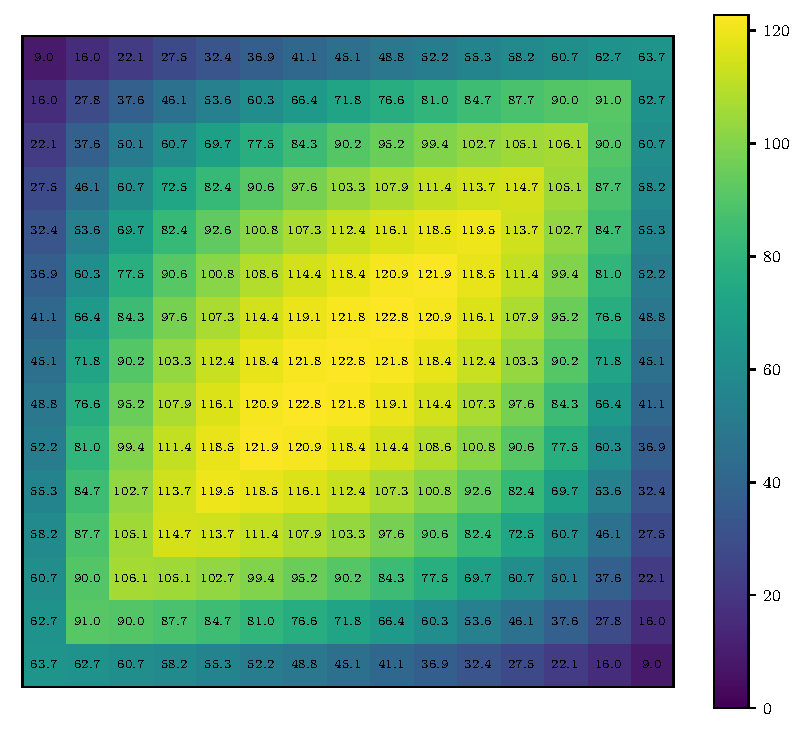
\includegraphics[width=\textwidth,keepaspectratio,clip]{rw-game/pvp_optimal_mean_times.pdf}
    \caption{
        Математическое ожидание числа ходов при оптимальной игре обоих игроков в случае PvP.
    }  
    \label{fig:optimal-value-pvp}
\end{figure}

Применяя формулы \cref{eq:game-2x2-prob} найдем вероятности выбора чистых стратегий в зависимости от положения на поле. Итоговые стратегии игроков при оптимальной игре приведены на рисунках \cref{fig:optimal-strategy-pvp-center,fig:optimal-strategy-pvp-border}. 

\begin{figure}[t]
    \centering
    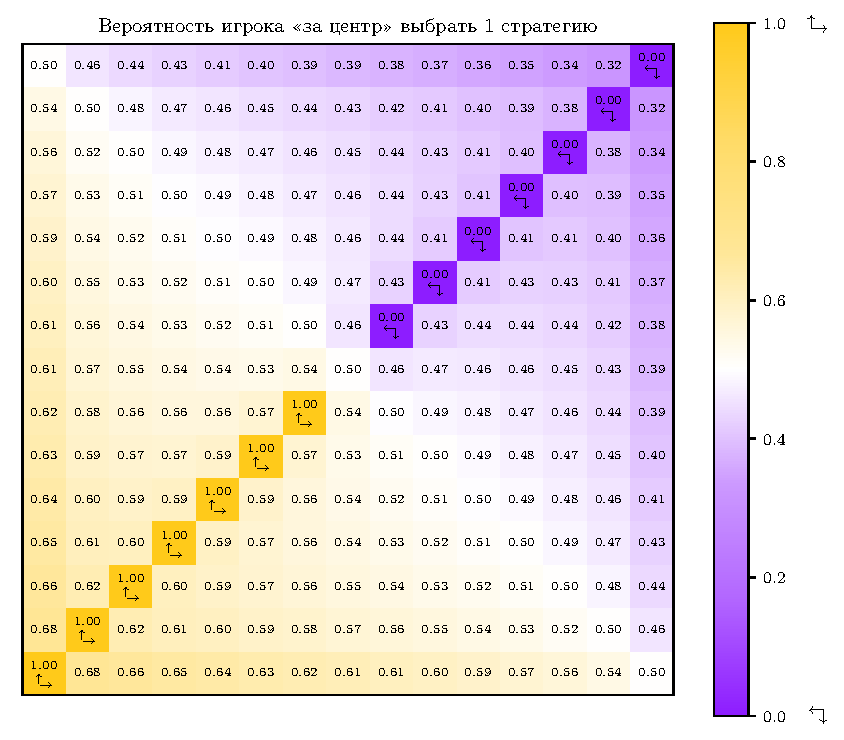
\includegraphics[width=\textwidth,keepaspectratio,clip]{rw-game/pvp_center_strategy.pdf}
    \caption{
        Оптимальная стратегия для игрока за центр в случае PvP.
    }  
    \label{fig:optimal-strategy-pvp-center}
    
\end{figure}

\begin{figure}[t]
    \centering
    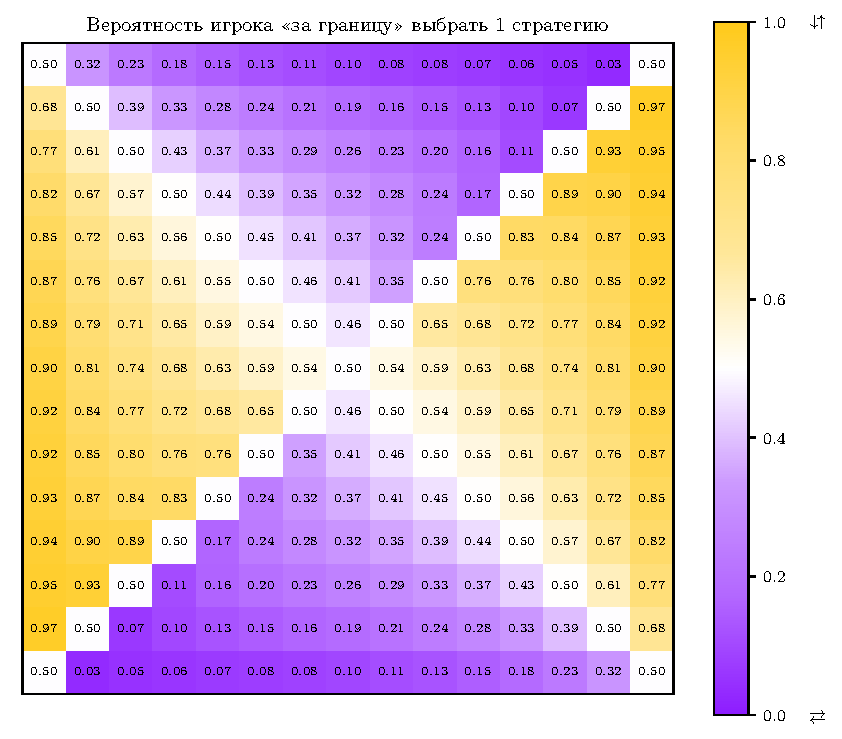
\includegraphics[width=\textwidth,keepaspectratio,clip]{rw-game/pvp_border_strategy.pdf}
    \caption{
        Оптимальная стратегия для игрока за границу в случае PvP.
    }  
    \label{fig:optimal-strategy-pvp-border}
    
\end{figure}

Рассмотрим подробнее получившиеся стратегии игроков. В отсутствии сопротивления от второго игрока, как в случае игры против бота, игрок за центр выбирает кнопку двигающую фишку в сторону диагонали. Находясь выше главной диагонали, соответственно игрок выбирает стратегию движения вниз-влево, а находясь ниже главной диагонали -- вверх-вправо. Добавление же второго игрока, оптимизирующего свою стратегию, заставляет первого игрока видоизменить свою стратегию, существенно уменьшив вероятности движения в сторону главной диагонали. Так, средняя вероятность выбора стратегии движения к главной диагонали, за исключением побочной диагонали, составляет всего $\approx 0.56$. Максимальная вероятность выбора стратегии движения к главной диагонали за исключением побочной диагонали, достигается в граничных узлах соседних с угловыми узлами побочной диагонали и составляет $\approx 0.68$. При удалении фишки от главной диагонали игрок за центр плавно увеличивает вероятность движения в сторону главной диагонали, при этом соотношение выбора стратегий изменяется от $1:1$ на главной диагонали до соотношения $\approx 3:2$ в пользу движения к главной диагонали. Выбор движения в центральном узле и на главной диагонали для игрока за центр не имеет значения, так как переходы из этих узлов приводят к симметричным играм. Движение же на побочной диагонали строго определено и должно осуществляться в направлении главной диагонали. Таким образом, стратегия игрока за центр интуитивно соответствует цели <<движения от границы>> с учетом большей рандомизации ходов.

Стратегии игрока за границу в сравнении с оптимальными стратегиями при игре против бота, напротив, имеют существенные различия. При игре против бота игрок за границу выбирает одно из направлений вертикальное или горизонтальное и всегда выбирает стратегию движения вдоль этого направления, никогда не пытаясь выбирать перпендикулярное направление параллельно ближайшей границе. Добавление в игру оппонента, оптимизирующего свою стратегию, игрок за границу попадает в ситуацию необходимости не демонстрировать свое намерение двигаться к границе, что заставляет его чаще выбирать движение параллельно ближайшей границе. Так средняя вероятность движения параллельно ближайшей границе за исключением побочной и главной диагоналей составляет $\approx 0.74$. Вблизи граничных узлов средняя вероятность достигает $\approx 0.87$, а максимальная вероятность $\approx 0.97$. Таким образом стратегия игрока за границу состоит в плавном увеличении вероятности движения параллельно ближайшей границе по мере приближения к ней. 


\section{Статистические свойства игры и сравнение с экспериментом}\label{sec:ch3/sec4}

Следующим шагом в анализе игровой динамики является сравнение результатов моделирования с результатами собранных игр в полевом эксперименте. Сбор траекторий в эксперименте осуществлялся с применением разработанной игры Random Walk Game и участием нескольких десятков людей. Подробное описание эксперимента приведено в разделе \cref{subsec:ch3/sec2/sub3} <<Полевой эксперимент с применением мобильных приложений и сети интернет>>. Суммарно в режиме PvE было собрано $1062$ игры: $528$ -- игры за центр, $534$ -- игры за границу. 

\subsection{Среднее время игры}\label{subsec:ch3/sec4/sub1}

Участники, цель которых была удерживать фишку как можно дольше внутри поля в среднем показали $145.45$ ходов за игру. Сравнивая этот результат с оптимальной стратегией, среднее время которой равно $\boldsymbol{\mathsf{t_{17}^{PvE A}}} = (17-2)^2 = 225$, получаем отставание на $54\%$ реальных игр от результатов моделирования. Хотя игроки показали не оптимальное время игры, выбранная ими стратегия позволяет улучшить в $2$ раза результат относительно $75.2$ хода в случае равновероятного выбора (BvB). Эксперимент показал, что рассматриваемая группа игроков способна распознать свойства игры и значительно улучшить среднее время игры несмотря на отсутствие априорного знания об оптимальной стратегии. В качестве подтверждения качества стратегии, найденной игроками, были получены относительные частоты для каждой позиции на поле и проведено моделирование столкновения стратегий случайного выбора против стратегии игроков. В результате моделирования было получено характерное среднее время игры $145.85$ согласующееся со средним временем экспериментальных траекторий.

Результаты игр участников в случае PvE с целью скорейшего достижения границы продемонстрировали среднее количество ходов равное $71.12$. В сравнении с оптимальной стратегией, среднее время которой равно $\boldsymbol{\mathsf{t_n^{PvE B}}} = \frac{(17-1)^2}{4} = 64$, игроки отстают на 7 ходов. Несмотря на такое отставание, среднее время игры у участников меньше на 4 хода, чем в случае равновероятного выбора. Аналогично предыдущему случаю игры за центр, игроки показали улучшение относительно случайного блуждания BvB и достаточно большой разрыв со средним временем игры для оптимальной стратегии. Моделирование игровой динамики за счет столкновения стратегий равновероятного случайного выбора и частот выборов, полученных из эксперимента, продемонстрировало отличие среднего времени игры, равного $73.79$, относительно среднего числа ходов в траекториях игроков. Предположительно, данное отличие вызвано неточными частотами в редко посещаемых состояниях. 

Результаты эксперимента корректно воспроизводятся при использовании частот из экспериментальных игр для случая PvE в качестве входных вероятностей для процесса моделирования с применением эволюции вероятности и численного моделирования отдельных траекторий. Таким образом, частоты выбора соответствующих стратегий, определенные для каждого состояния, позволили нам интерпретировать множество $f_{ij}$ как усредненную стратегию, найденную группой участников эксперимента. Значения среднего времени игры представлены в сводной таблице (см. Таблицу~\cref{tab:time}).

\begin{table}
    \fontsize{10pt}{10pt}\selectfont
    \begin{tabular}{|l|c|c|c|c|c|}
        \toprule
        Размер поля $17 \times 17$ & \textbf{BvB} & \textbf{PvE центр} & \textbf{PvE граница} & \textbf{PvP} & \textbf{PvP $400+$} \\ 
        \midrule
        \textbf{Количество игр} & -     & 528    & 534   & 500    & 13     \\
        \midrule
        \textbf{Эксперимент}  & -     & 145.45 & 71.12 & 120.60 & 594.27 \\ 
        \textbf{Моделирование траекторий}  & 75.22 & 145.77 & 73.66 & 115.93 & 132.91 \\
        \textbf{Теория Марковских цепей}  & 75.21 & 145.85 & 73.79 & 116.22 & 133.22 \\
        \textbf{Эволюция вероятности}   & 75.21 & 145.85 & 73.79 & 116.22 & 133.22 \\ 
        \textbf{Оптимальная стратегия}     & -     & 225.00 & 64.00 & 122.8  & -      \\ 
        \bottomrule
    \end{tabular}
    \caption{
        Средние времена поглощения, полученные с применением различных подходов для 4 случаев игры: BvB -- чистое случайное блуждание на квадратной решетке с поглощением на границе, PvE -- случай игры против стратегии равновероятного выбора с двумя целями: центр -- цель оставаться как можно дольше внутри поля, граница -- цель как можно скорее достичь границы, случай PvP -- игры двух игроков с произвольными стратегиями, случай PvP 400+ -- игры двух игроков, имеющие количество ходов свыше 400. Значения представлены для поля размером $17 \times 17$. При моделировании траекторий использовалось $10^5$ запусков для сбора статистики. Моделирование эволюции вероятности происходило в течение первых $10^4$ шагов. Моделирование траекторий, теория поглощающих Марковских цепей и эволюция вероятности были выполнены на основе частот, полученных в реальных играх в полевом эксперименте. Для случая BvB частоты стратегий игроков выбирались по 0.5 (равновероятный выбор одной из кнопок).
    }
    \label{tab:time}
\end{table}

Среднее время игр участников друг с другом (PvP) находится между средними временами поглощения для случаев PvE при игре за центр и при игре за границу. Среднее количество ходов в PvP-играх на 57 ходов больше, чем среднее время игры в оптимальной стратегии PvE с пограничной целью. Сравнение с режимом PvE за центр показывает на 25 ходов меньше среднее время игры в PvP по сравнению с экспериментальными играми PvE и примерно в 2 раза меньше в PvP по сравнению с оптимальной стратегией при игре за центр в случае PvE.

Среднее время поглощения, полученное путем моделирования для конкретных частот, совпадает со средним значением теории AMC (абсолютная ошибка составила менее $10^{-9}$). Таким образом, оба метода могут применяться для точного вычисления среднего времени поглощения для произвольных стратегий. Подход к моделированию траекторий $10^5$ показывает точность до целой части значения среднего времени игры.

Для удобства сравнения средних времен приводится столбчатая диаграмма, демонстрирующая различные стратегии игроков \cref{fig:mean-times}. Тривиальная совместная стратегия игроков, минимизирующая время игры, состоит в выборе на всех ходах одной и той же чистой стратегии, среди двух предложенных. Выбор конкретной чистой стратегии не играет роли, так как независимо от него фишка будет двигаться в направлении к границе и достигнет ее за 8 ходов. 

Сравнение оптимальной стратегии игроков в случае PvP и экспериментально полученного среднего времени игры демонстрирует разницу менее двух ходов с небольшим отставанием популяционной стратегии. Такое сходство подтверждает высокую предсказательную силу предложенной модели для описания статистических свойств игры.

\begin{figure}[t]
    \centering
    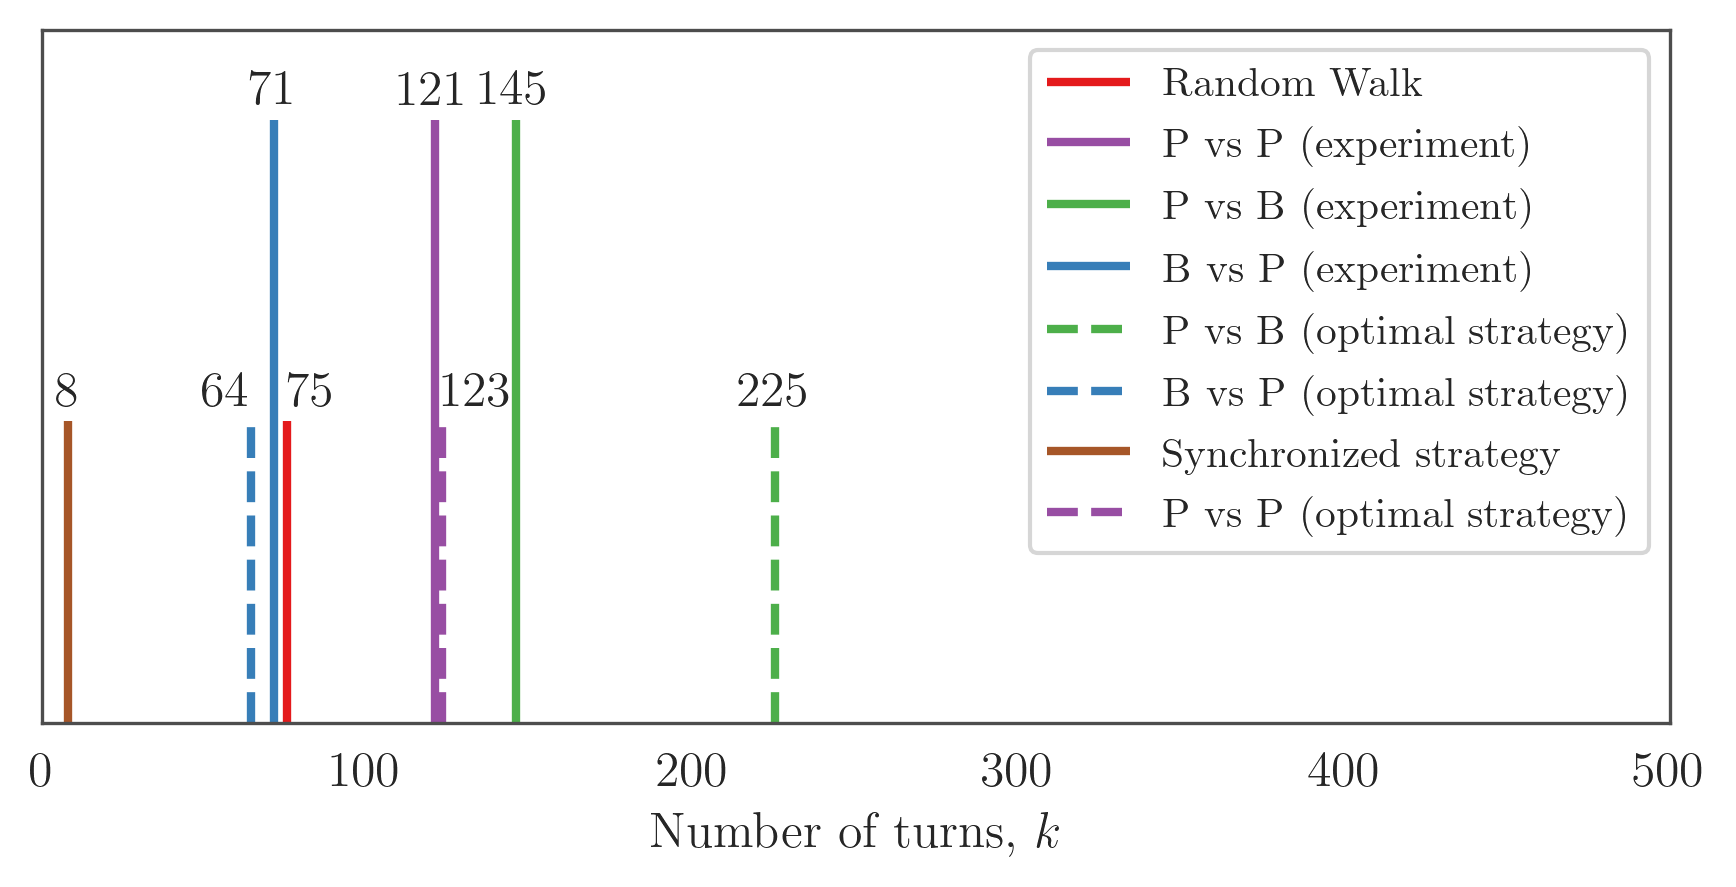
\includegraphics[width=\textwidth,keepaspectratio,clip]{rw-game/fig2p_v3.png}
    \caption{
        Среднее время игры, полученное в эксперименте, в сравнении с различными стратегиями и чистым случайным блужданием.
    }  
    \label{fig:mean-times}
\end{figure}


\subsection{Четность времени игры}\label{subsec:ch3/sec4/sub2}

Моделирование игрового процесса позволило идентифицировать различия между четной и нечетной продолжительностью игры. Для анализа четности вычислим вероятность закончить игру при четном и нечетном количестве ходов. Результаты представлены в Таблице~\cref{tab:parity}. Экспериментальные результаты в PvE за границу показывают почти равные частоты окончаний на четных и нечетных ходах. Однако в случае игр за центр вероятность закончить на нечетном ходу в $2$ раза выше, чем на четном. Аналогичное поведение было обнаружено в режиме PvP. Эти результаты указывают на склонность игроков к завершению игры в нечетных состояниях (то есть состояний в которых нечетная сумма координат). Хотя нечетные поглощающие состояния наблюдаются чаще, примерно $30\%$ игр заканчиваются четными состояниями. Это, в свою очередь, показывает необходимость наличия ненулевой вероятности как нечетных, так и четных окончаний в соответствующих играх между двумя игроками.

В отличие от игры двух игроков, оптимальные стратегии для режимов PvE демонстрируют явное предпочтение четным концовкам в случае игры за границу и нечетным концовкам в случае игры за центр. Первый раз граничные состояния поля могут быть достигнуты за $8$ ходов или $\frac{n-1}{2}$ для произвольного размера поля, что соответствует четным количествам ходов ($n$ -- нечетное). Вероятность такого события для оптимальной стратегии равна $0.00815$ на поле размером $17 \times 17$. Возможность удерживать фишку внутри поля с вероятностью единица доступна только для первых $14$ ходов, и на $15$-м ходу она будет поглощена с вероятностью приблизительно $0.000061$ в поле $17 \times 17$. В общем случае, поглощение произойдет с ненулевой вероятностью на нечетном $n-2$ ходу.

\begin{table}[t]
    \fontsize{10pt}{10pt}\selectfont
    \begin{tabular}{|l|c|c|c|c|c|}
        \toprule
        Размер поля $17 \times 17$ & \textbf{BvB} & \textbf{PvE центр} & \textbf{PvE граница} & \textbf{PvP} & \textbf{PvP $400+$} \\
        \midrule
        \textbf{Эксперимент} & --     & 30:70 & 51:49 & 35:65 & 15:84 \\
        \textbf{Моделирование траекторий} & 50:50 & 30:70 & 51:49 & 36:64 & 31:69 \\
        \textbf{Эволюция вероятности}  & 50:50 & 30:70 & 51:49 & 36:64 & 31:69 \\
        \textbf{Оптимальная стратегия*}    & --     & 0:100 & 100:0 & --   & --     \\
        \bottomrule
    \end{tabular}
    \caption{
        Отношение шансов закончить игру при четном числе ходов к нечетному (четное~$:$~нечетное). Значения были получены разными подходами для 4 случаев игры: BvB -- чистое случайное блуждание по двумерной конечной решетке, PvE -- случай игры против стратегии равновероятного выбора с двумя целями: центр -- цель оставаться как можно дольше внутри поля, граница -- цель как можно скорее достичь границы, случай PvP -- игры двух игроков с произвольными стратегиями, случай PvP 400+ -- игры двух игроков, имеющие количество ходов свыше 400. Значения представлены для поля размером $17 \times 17$. При моделировании траекторий использовалось $10^5$ запусков для сбора статистики. Моделирование эволюции вероятности происходило в течение первых $10^4$ шагов. Моделирование траекторий, теория поглощающих Марковских цепей и эволюция вероятности были выполнены на основе частот, полученных в реальных играх в полевом эксперименте. Для случая BvB частоты стратегий игроков выбирались по $0.5$ (равновероятный выбор одной из кнопок).
    }
    \label{tab:parity}
\end{table}

\subsection{Распределение времен игры}\label{subsec:ch3/sec4/sub3}

Моделирование эволюции вероятностей и траекторий позволили вычислить точные и приближенные вероятности завершения игры на $k$-ом ходе. Применение этих методов требует определения конкретной смешанной стратегии в зависимости от положения на игровом поле. Случай BvB чистого случайного блуждания определяет простую стратегию равновероятного выбора из двух доступных вариантов независимо от положения на игровом поле. Дополнительно к экспериментальным данным были проанализированы две предложенные стратегии оптимального случайного блуждания в режиме PvE. Помимо аналитических стратегий были получены экспериментальные частоты выбора стратегий в каждом состоянии. На основе этих стратегий было проведено моделирование эволюции вероятности по игровому полю во времени, а также моделирование индивидуальных траекторий с использованием различных стратегий ($10^5$ реализаций на каждый случай). В результате были получены распределения времен поглощения, представленные на Рис.~\cref{fig:distribution_time}.

\begin{figure*}[t]
    \centering
    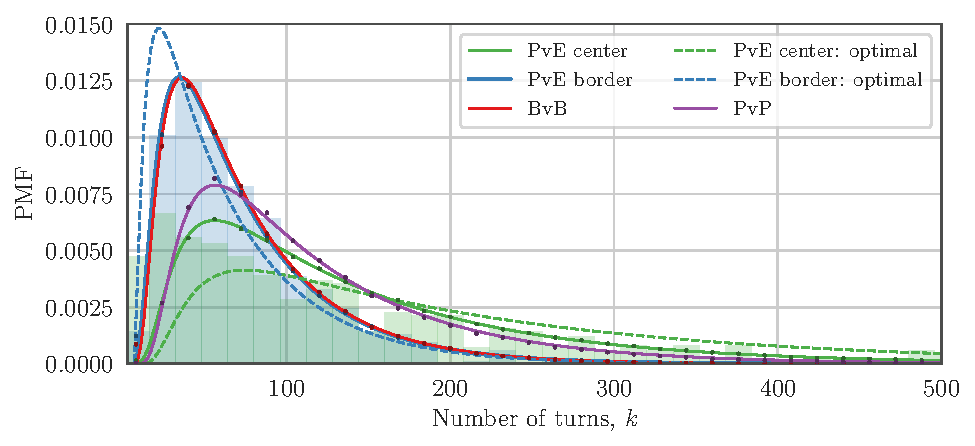
\includegraphics[width=\textwidth,keepaspectratio,clip]{rw-game/fig3.pdf}
    \caption{
        Распределение количества ходов, полученное моделированием эволюции вероятности (сплошная линия) и численным моделированием (точки) с использованием соответствующих стратегий игроков A и B. Режим BvB (красная линия) представляет собой равновероятный выбор для обоих игроков. Кривые PvE (зеленый и синий) и PvP-режим (фиолетовая линия) были построены на основе соответствующих усредненных стратегий по популяции. Противоположная стратегия в режиме PvE -- это стратегия равновероятного выбора. Оптимальная стратегия для режима PvE в центре (зеленая пунктирная линия) -- держать фишку на диагональной лестнице. Оптимальная стратегия для режима границы PvE (синяя пунктирная линия) -- выбирать движения только вдоль горизонтальной линии. Гистограммы, полученные экспериментально, представлены для режимов PvE (зеленая и синяя области).
    }  
    \label{fig:distribution_time}
    
\end{figure*}

При детальном рассмотрении у всех распределений наблюдаются различия в вероятностях на четных и нечетных ходах. Для оценки характерного поведения распределений, рассмотрим гистограмму с широкими интервалами (длиной в $16$ ходов). Анализ показывает, что все режимы игры следуют одному и тому же паттерну:
\begin{itemize}
\item короткие партии встречаются редко;
\item распределение имеет одну моду с промежуточным числом ходов;
\item вероятность длинных игр экспоненциально уменьшается с увеличением длины игры.
\end{itemize}

Режим PvE за центр демонстрирует аналогичную форму распределения, за исключением того, что мода соответствует коротким играм, которая скрыта при отображении с выбранным размером интервалов.

Хотя количество собранных траекторий в режиме PvP ($500$) не очень большое, в распределении наблюдались нехарактерно долгие игры с длиной более $400$ ходов. Вероятность получения таких игр согласно моделированию средней популяционной стратегии ниже $0.015$. Однако в играх участников было обнаружено $13$ длинных траекторий в диапазоне от $461$ до $964$ ходов со средним временем поглощения равным $594.27$. Обнаруженное отклонение можно объяснить <<синхронизацией>> между отдельными индивидуумами при длительном взаимодействии. Поскольку в среднем один ход занимает $4.5$ секунды, игра с $400$ ходами длится $30$ минут. Такое продолжительное время, в течение которого игрок B не может завершить игру, вызывает разочарование и снижает концентрацию. Это в свою очередь может привести к бессознательному принятию решений, которые может легко предсказать игрок A. Потеря концентрации приводит к ухудшению способности человека производить выбор стратегий случайным образом. В связи с этим в игре могут возникать процессы <<синхронизации>>.

Подробный анализ этих игр был выполнен путем отделения стратегий этих игр от основной части распределения. В результате моделирования столкновения противоположных стратегий для случая PvP 400+ было получено меньшее среднее время поглощения, составившее приблизительно $133.22$ ходов. Чтобы сравнить распределения таких игр, также было проведено моделирование эволюции вероятностей для частот, наблюдавшихся в стратегиях длительных игр. Соответствующие распределения, полученные для длинных игр, изображены на Рис.~\cref{fig:distribution_time_PvP}. Хотя распределение частот демонстрирует длинный хвост, лежащие в основе стратегии, которые появляются в <<синхронизированных>> играх, не воспроизводят появление столь же длинных игр. Таким образом, это демонстрирует наличие зависимости выбора игроков от скрытых факторов, которые нельзя объяснить только свойством цепи Маркова.

\begin{figure*}[t]
    \centering
    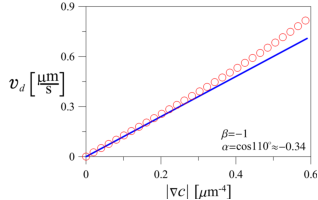
\includegraphics[width=\textwidth,keepaspectratio,clip]{rw-game/fig4.pdf}
    \caption{
        Распределение времени поглощения для режима PvP (желтая гистограмма и фиолетовая линия) по сравнению с моделированием частот направлений движения (зеленая линия) и частот стратегий (синяя линия), наблюдаемых в длительных играх (более $400$ ходов). Частоты направлений движения для каждого состояния, полученные в экспериментальных длинных играх, использовались для моделирования эволюции вероятностей найти фишку в узлах решетки. Стратегии обоих игроков A и B в PvP с длиной ходов более $400$ использовались отдельно при моделировании.
    }  
    \label{fig:distribution_time_PvP}

\end{figure*}

\subsection{Пространственное распределение}\label{subsec:ch3/sec4/sub4}

Затем была проанализирована вероятность нахождения фишки в определенном состоянии во время игры. Как и в предыдущих разделах, проведено сравнение экспериментально полученных частот и результатов моделирования. Визуализации пространственных распределений для соответствующих стратегий изображены на Рис.~\cref{fig:distribution_states}.

\begin{figure}[t]
    \centering
    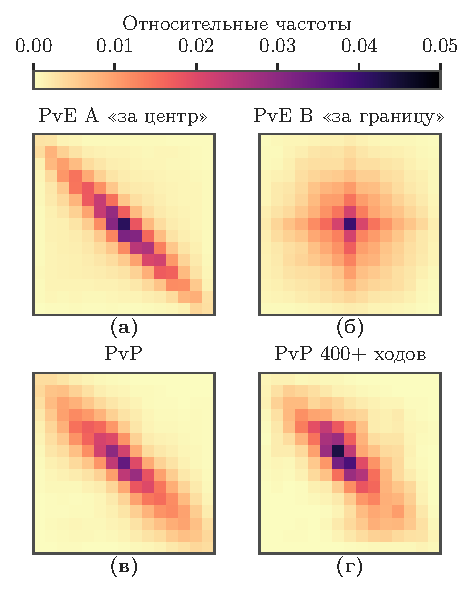
\includegraphics[width=\columnwidth,keepaspectratio,clip]{rw-game/fig5.pdf}
    \caption{
        Двухмерные распределения частоты посещений узлов решетки, полученные в экспериментальных играх для 4 случаев: 
        PvE за центр, PvE за границу, игры двух игроков (PvP) и игры продолжительностью более $400$ ходов в режиме PvP.
    }  
    \label{fig:distribution_states}
    
\end{figure}

Чистое случайное блуждание демонстрирует дискретное гауссово распределение в пространстве. Добавление игровой динамики в свою очередь меняет итоговую картину распределения. Как и следовало ожидать, режим PvE в играх за центр демонстрирует в основном движения по диагонали (см. Рис.~\cref{fig:distribution_states}A). Хотя это поведение совпадает с пространственным распределением в предложенной оптимальной стратегии, экспериментальные данные имеют больший разброс вокруг диагональных состояний, чем для оптимальной стратегии.

Оптимальная стратегия в случае игры PvE за границу демонстрирует вертикальные или горизонтальные линии состояний, по которым происходит перемещение фишки. В результате экспериментальных игр PvE за границу найдены 3 основных паттерна в распределении (см. Рис.~\cref{fig:distribution_states}B): ожидаемые движения по прямым линиям, и отличное движение от оптимального паттерна -- это распределение, похожее на чистое случайное блуждание на двумерной квадратной решетке. Второй паттерн показывает попытку популяции найти стратегию в двумерном пространстве лучше, чем на одномерной линии. Однако уход одномерных отрезков увеличивает среднее время поглощения. Это объясняет небольшую разницу в средних временах поглощения между экспериментальным играми в случае PvE за границу и чистым случайным блужданием BvB.

Схема пространственного распределения в случае игры PvP (см. Рис.~\cref{fig:distribution_states}C) аналогична случаю PvE при игре за центр: фишка в основном движется по диагонали. Единственное отличие -- увеличенный разброс относительно диагональной линии, который показывает более сильную усредненную стратегию для игрока B (цель достичь границу), по сравнению с равновероятным случайным выбором (как в случае игры PvE за центр). Дополнительной характерной особенностью случая PvP является более яркая выраженность блужданий в левой верхней и правой нижней четвертях квадрата относительно центра, в сравнении со случаем PvE при игре за центр. Посещение же двух других четвертей квадрата является более редким событием.

В заключение, было проанализировано пространственное распределение состояний в играх длиной более $400$ ходов. Вероятность расположения фишки в основном сосредоточена на главной диагонали, как и в предыдущих случаях (см. Рис.~\cref{fig:distribution_states}D). Тем не менее распределение более компактно в центре поля и имеет более высокую вариацию вокруг главной диагонали по сравнению со случаями PvE за центр и PvP. Такое поведение предполагает более длительное нахождение фишки ближе к центру в длинных партиях с движением не только по диагонали, а также перпендикулярно ей.

\subsection{Анализ стратегий}\label{subsec:ch3/sec4/sub5}

Далее, рассмотрим сравнение усредненных стратегий популяции для игроков A и B друг с другом, а также с оптимальными стратегиями. Для представления стратегий, визуализируем их в виде цветной двумерной матрицы с элементами, соответствующими состояниям на двумерной квадратной решетке (Рис.~\cref{fig:strategies}). Цвет элемента матрицы отображает частоту выбора первой кнопки из двух возможных вариантов в соответствии с правилами (см. Рис.~\cref{fig:controls}). Игрок А, старающийся сохранять фишку внутри поля, имеет два варианта: двигаться вверх/вправо или двигаться вниз/влево; игрок B старающийся как можно скорее достичь границы имеет также два выбора: двигаться вверх/вниз или двигаться влево/вправо. Разные цвета элементов матрицы демонстрируют, какой из двух выборов доминирует для каждого состояния в среднем по всем играм популяции.

\begin{figure*}[t]
    \centering
    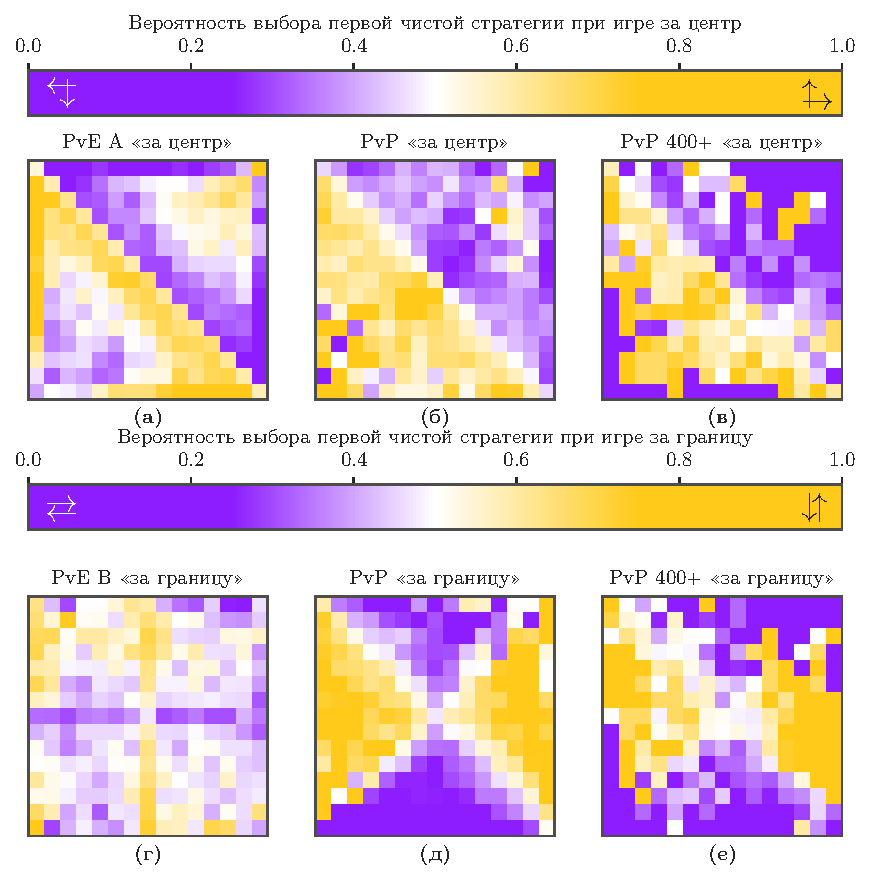
\includegraphics[width=\textwidth,keepaspectratio,clip]{rw-game/fig6.pdf}
    \caption{
        Визуализация средних популяционных стратегий для разных режимов, полученных в эксперименте. Цвет ячеек отображает частоту выбора первой чистой стратегии: для игры за центр (A, B, C) и для игры за границу (D, E, F).
    }  
    \label{fig:strategies}
    
\end{figure*}

Стратегия, наблюдаемая в случае режима PvE за центр, демонстрирует в основном движение в направлении диагональных состояний (Рис.~\cref{fig:strategies}A). Однако состояния, удаленные от диагонали, показывают немного более высокие частоты противоположных стратегий. Обычно игроки выбирают уходить от границы, но в состояниях ближе к углам на боковой диагонали поведение становится более случайным (относительные частоты ближе к $0.5$). Экспериментальная стратегия на главной диагонали демонстрирует схожесть с первой оптимальной стратегией, рассмотренной в разделе \cref{subsec:ch3/sec3/sub4} <<Решение задачи поиска оптимальных стратегий>>. Напротив, выбор игроков на границе отличается от второй оптимальной стратегии, которая предлагает всегда двигаться в направлении от границы. Это приводит к утечке вероятностей за пределы поля не только в углах главной диагонали, но и в других пограничных состояниях, что в свою очередь значительно снижает среднее время игры. 

Стратегия игрока, играющего за центр, в случае PvP аналогична стратегии PvE для игрока за центр (Рис.~\cref{fig:strategies}B). Более того, в среднем игроки предпочитают двигаться в направлении главной диагонали независимо от положения на решетке. Почти все состояния вблизи границы демонстрируют аналогичную стратегию, за исключением некоторых состояний с почти равной частотой обоих вариантов. По сравнению с режимом PvE за центр, игрок в случае PvP играющий за центр имеет немного меньшую уверенность в движении к главной диагонали (частоты ближе к $0.5$ в PvP по сравнению с PvE).

Стратегия PvE за границу четко определена на горизонтальной и вертикальной линиях (Рис.~\cref{fig:strategies}D). Хотя игроки чаще выбирают движение к ближайшей границе на центральных прямых, частоты в других состояниях не соответствуют общей схеме. В отличие от схожих стратегий PvE и PvP в случае игры за центр, стратегия PvP при игре за границу демонстрирует отличающееся поведение с четко прослеживаемым паттерном (Рис.~\cref{fig:strategies}E). В этом случае игроки действуют прямо противоположно режиму PvE за границу. Усредненная стратегия популяции предлагает выбирать движение по координатной линии имеющей наименьшее отклонение от центра. В результате плоскость решений разбивается на $4$ чередующихся треугольника. Хотя частоты близки к $0$ или $1$, имеется небольшая разница, которая свидетельствует о редких попытках движения к ближайшей границе. Такое значительное отличие предположительно связано с очевидностью для игрока за центр выбора оппонента перемещаться в направлении границы. Это заставляет игрока старающегося достичь границу реже делать попытки перемещения к границе для уменьшения шансов предсказать и противодействовать этому движению со стороны второго игрока.

Для результирующих стратегий, полученных в длинных играх между двумя игроками (Рис.~\cref{fig:strategies}C,F), четких закономерностей не наблюдается из-за ограниченного количества игр. Однако наблюдается сходство принципов принятия решений с обычным случаем PvP.

\section{Оценка когнитивного статуса при возрастных изменениях}\label{sec:ch3/sec5}

В предыдущих разделах были рассмотрены математические аспекты игры, позволяющие обнаружить оптимальные стратегии. Однако игроки, продемонстрировали результат, отличающийся от оптимального для некоторых случаев игры, а также были найдены некоторые сверхдлинные игры, не укладывающиеся в марковскую модель. Влияние различных факторов на способность игроков-людей оптимально принимать решения в течение длительного времени привносит в игру дополнительную неопределенность. Способность к концентрации внимания и способность быстро и эффективно принимать решения в условиях игры зависит от когнитивного статуса индивидуума, возраста, наличия когнитивных нарушений, утомления и психологии индивидуума. Анализ комбинации всех перечисленных свойств индивидуума представляет собой комплексную задачу, требующую проведение множества психофизиологических экспериментов, сбор статистических данных, построение математических моделей для анализа собранных данных и построение результирующей нелинейной модели для оценки текущего состояния с учетом множества факторов. Наличие такого инструмента позволит в дальнейшем контролировать игровой эксперимент и исключать перечисленные факторы. 

Одним из важных аспектов, влияющих на способность принимать решения являются возраст-зависимые изменения в организме человека. Когнитивный статус, включая память, мышление, двигательные реакции и внимание, а также скорость обработки информации, играет центральную роль в здоровом старении. Когнитивный спад является причиной многих трудностей даже в повседневной жизни, влияющих на самочувствие человека. Снижение эффективности принятия решений у пожилых людей объясняется когнитивными ограничениями в обработке информации \cite{frey_role_2015}, а также непоследовательностью своих выборов \cite{finucane_task_2005}. В работах по исследованию возрастных изменений головного мозга на клеточном и системном уровнях была предложена концепция <<когнитивного старения>> \cite{blazer_cognitive_2017}.

Используя когнитивные тесты, предложенные исследователями кафедры нейропсихофизиологии ННГУ им.~Н.И~Лобачевского, а также экспериментальные и организационные возможности ИББМ ННГУ им.~Н.И.~Лобачевского, был получен набор данных с информацией о результатах когнитивных тестах, возрасте и поле испытуемых. Когорта испытуемых состояла из 118 человек (37 мужчин и 81 женщина) в возрасте от 19 до 85 лет. В исследовании применялись три когнитивных теста: два сенсомоторных теста (SM1, SM2) и тест кампиметрии (CM). Выбранные тесты позволили охарактеризовать когнитивный статус пациентов с учетом возникающих возрастных изменений \cite{polevaya_eventrelated_2019}. В рамках исследования на основе моделей машинного обучения были построены когнитивные часы, позволяющие определить ускорение когнитивного возраста относительно хронологического возраста индивидуума. Такой интегральный показатель характеризует суммарный вклад рассматриваемых когнитивных показателей в когнитивный статус. С применением методов кластеризации и объяснимого искусственного интеллекта было получено разложение интегрального показателя когнитивного возраста на составляющие, демонстрирующие вклад отдельных когнитивных характеристик в предсказание модели. 

Наиболее качественные результаты были получены с применением машины опорных векторов с радиальным ядром, позволяющим учесть нелинейность взаимосвязей между признаками. Используя корреляционный анализ, 64 показателя были упорядочены по уровню корреляции с возрастом. Оценка качества работы алгоритма машинного обучения при последовательном наборе признаков позволила выделить 24 наилучших показателя, дающих наименьшую кроссвалидационную ошибку при оценке возраста. При оптимальном выборе коэффициент детерминации $R^2$ качества оценки регрессии составил 0.52. Наиболее релевантными признаками в модели оказались времена прохождения теста кампиметрии, количество оттенков, необходимых для распознавания образа, доля некорректно определенных арифметических выражений и моторная реакция в тесте на зеркальные буквы. 

Для подтверждения биологической релевантности результата полученные когнитивные часы и соответствующие показатели были сопоставлены корреляционным анализом с биологическим возрастом индивидуума. Построение аналогичных часов при обучении с биологическим и эпигенетическим возрастами в качестве целевой переменной выявило статистически меньшую ошибку при предсказании. Такой результат демонстрирует вклад когнитивного статуса индивидуума в его эпигенетический возраст, вычисленный по различным моделям \cite{levine_epigenetic_2018,horvath_dna_2013,lu_dna_2019}.

Результаты исследования опубликованы в работе \cite{bib4}, а также апробированы на конференциях \cite{confbib2,confbib3}. Получено свидетельство о государственной регистрации программы для ЭВМ \cite{progbib2}.
 

\section{Выводы по главе 3}\label{sec:ch3/sec6}

В данной главе были рассмотрены основные результаты сравнения статистических свойств экспериментально полученных траекторий и стратегий игроков с соответствующими результатами моделирования различными подходами. Предложена гипотеза об оптимальных средних временах достижения границы для двух случаев игры и рассмотрены соответствующие стратегии, достигающие оптимальных времен. Продемонстрирована оптимальность данных стратегий и средних времен игры для случаев малого размера поля. Гипотеза об оптимальных средних временах была подтверждена решением игры на основе теории рекурсивных игр. Приведены расчеты оптимальных средних времен игры и оптимальных стратегий для третьего случая игры двух оппонентов, оптимизирующих свои стратегии. В главе для анализа игры Random Walk Game применены подходы теории игр, численного моделирования, моделирования эволюции вероятности и полевого эксперимента, на основе которых вычислены средние времена игры, распределения времен игры и пространственные распределения фишки на поле. Полученные результаты визуализированы с использованием языка Python 3.8 и библиотек numpy, scipy, matplotlib. 